% Options for packages loaded elsewhere
\PassOptionsToPackage{unicode}{hyperref}
\PassOptionsToPackage{hyphens}{url}
%
\documentclass[
]{book}
\usepackage{lmodern}
\usepackage{amssymb,amsmath}
\usepackage{ifxetex,ifluatex}
\ifnum 0\ifxetex 1\fi\ifluatex 1\fi=0 % if pdftex
  \usepackage[T1]{fontenc}
  \usepackage[utf8]{inputenc}
  \usepackage{textcomp} % provide euro and other symbols
\else % if luatex or xetex
  \usepackage{unicode-math}
  \defaultfontfeatures{Scale=MatchLowercase}
  \defaultfontfeatures[\rmfamily]{Ligatures=TeX,Scale=1}
\fi
% Use upquote if available, for straight quotes in verbatim environments
\IfFileExists{upquote.sty}{\usepackage{upquote}}{}
\IfFileExists{microtype.sty}{% use microtype if available
  \usepackage[]{microtype}
  \UseMicrotypeSet[protrusion]{basicmath} % disable protrusion for tt fonts
}{}
\makeatletter
\@ifundefined{KOMAClassName}{% if non-KOMA class
  \IfFileExists{parskip.sty}{%
    \usepackage{parskip}
  }{% else
    \setlength{\parindent}{0pt}
    \setlength{\parskip}{6pt plus 2pt minus 1pt}}
}{% if KOMA class
  \KOMAoptions{parskip=half}}
\makeatother
\usepackage{xcolor}
\IfFileExists{xurl.sty}{\usepackage{xurl}}{} % add URL line breaks if available
\IfFileExists{bookmark.sty}{\usepackage{bookmark}}{\usepackage{hyperref}}
\hypersetup{
  pdftitle={Survey Data: Design and Examples},
  pdfauthor={Ehsan Karim},
  hidelinks,
  pdfcreator={LaTeX via pandoc}}
\urlstyle{same} % disable monospaced font for URLs
\usepackage{color}
\usepackage{fancyvrb}
\newcommand{\VerbBar}{|}
\newcommand{\VERB}{\Verb[commandchars=\\\{\}]}
\DefineVerbatimEnvironment{Highlighting}{Verbatim}{commandchars=\\\{\}}
% Add ',fontsize=\small' for more characters per line
\usepackage{framed}
\definecolor{shadecolor}{RGB}{248,248,248}
\newenvironment{Shaded}{\begin{snugshade}}{\end{snugshade}}
\newcommand{\AlertTok}[1]{\textcolor[rgb]{0.94,0.16,0.16}{#1}}
\newcommand{\AnnotationTok}[1]{\textcolor[rgb]{0.56,0.35,0.01}{\textbf{\textit{#1}}}}
\newcommand{\AttributeTok}[1]{\textcolor[rgb]{0.77,0.63,0.00}{#1}}
\newcommand{\BaseNTok}[1]{\textcolor[rgb]{0.00,0.00,0.81}{#1}}
\newcommand{\BuiltInTok}[1]{#1}
\newcommand{\CharTok}[1]{\textcolor[rgb]{0.31,0.60,0.02}{#1}}
\newcommand{\CommentTok}[1]{\textcolor[rgb]{0.56,0.35,0.01}{\textit{#1}}}
\newcommand{\CommentVarTok}[1]{\textcolor[rgb]{0.56,0.35,0.01}{\textbf{\textit{#1}}}}
\newcommand{\ConstantTok}[1]{\textcolor[rgb]{0.00,0.00,0.00}{#1}}
\newcommand{\ControlFlowTok}[1]{\textcolor[rgb]{0.13,0.29,0.53}{\textbf{#1}}}
\newcommand{\DataTypeTok}[1]{\textcolor[rgb]{0.13,0.29,0.53}{#1}}
\newcommand{\DecValTok}[1]{\textcolor[rgb]{0.00,0.00,0.81}{#1}}
\newcommand{\DocumentationTok}[1]{\textcolor[rgb]{0.56,0.35,0.01}{\textbf{\textit{#1}}}}
\newcommand{\ErrorTok}[1]{\textcolor[rgb]{0.64,0.00,0.00}{\textbf{#1}}}
\newcommand{\ExtensionTok}[1]{#1}
\newcommand{\FloatTok}[1]{\textcolor[rgb]{0.00,0.00,0.81}{#1}}
\newcommand{\FunctionTok}[1]{\textcolor[rgb]{0.00,0.00,0.00}{#1}}
\newcommand{\ImportTok}[1]{#1}
\newcommand{\InformationTok}[1]{\textcolor[rgb]{0.56,0.35,0.01}{\textbf{\textit{#1}}}}
\newcommand{\KeywordTok}[1]{\textcolor[rgb]{0.13,0.29,0.53}{\textbf{#1}}}
\newcommand{\NormalTok}[1]{#1}
\newcommand{\OperatorTok}[1]{\textcolor[rgb]{0.81,0.36,0.00}{\textbf{#1}}}
\newcommand{\OtherTok}[1]{\textcolor[rgb]{0.56,0.35,0.01}{#1}}
\newcommand{\PreprocessorTok}[1]{\textcolor[rgb]{0.56,0.35,0.01}{\textit{#1}}}
\newcommand{\RegionMarkerTok}[1]{#1}
\newcommand{\SpecialCharTok}[1]{\textcolor[rgb]{0.00,0.00,0.00}{#1}}
\newcommand{\SpecialStringTok}[1]{\textcolor[rgb]{0.31,0.60,0.02}{#1}}
\newcommand{\StringTok}[1]{\textcolor[rgb]{0.31,0.60,0.02}{#1}}
\newcommand{\VariableTok}[1]{\textcolor[rgb]{0.00,0.00,0.00}{#1}}
\newcommand{\VerbatimStringTok}[1]{\textcolor[rgb]{0.31,0.60,0.02}{#1}}
\newcommand{\WarningTok}[1]{\textcolor[rgb]{0.56,0.35,0.01}{\textbf{\textit{#1}}}}
\usepackage{longtable,booktabs}
% Correct order of tables after \paragraph or \subparagraph
\usepackage{etoolbox}
\makeatletter
\patchcmd\longtable{\par}{\if@noskipsec\mbox{}\fi\par}{}{}
\makeatother
% Allow footnotes in longtable head/foot
\IfFileExists{footnotehyper.sty}{\usepackage{footnotehyper}}{\usepackage{footnote}}
\makesavenoteenv{longtable}
\usepackage{graphicx,grffile}
\makeatletter
\def\maxwidth{\ifdim\Gin@nat@width>\linewidth\linewidth\else\Gin@nat@width\fi}
\def\maxheight{\ifdim\Gin@nat@height>\textheight\textheight\else\Gin@nat@height\fi}
\makeatother
% Scale images if necessary, so that they will not overflow the page
% margins by default, and it is still possible to overwrite the defaults
% using explicit options in \includegraphics[width, height, ...]{}
\setkeys{Gin}{width=\maxwidth,height=\maxheight,keepaspectratio}
% Set default figure placement to htbp
\makeatletter
\def\fps@figure{htbp}
\makeatother
\setlength{\emergencystretch}{3em} % prevent overfull lines
\providecommand{\tightlist}{%
  \setlength{\itemsep}{0pt}\setlength{\parskip}{0pt}}
\setcounter{secnumdepth}{5}
\usepackage{booktabs}
\usepackage{amsthm}
\makeatletter
\def\thm@space@setup{%
  \thm@preskip=8pt plus 2pt minus 4pt
  \thm@postskip=\thm@preskip
}
\makeatother
\usepackage[]{natbib}
\bibliographystyle{apalike}

\title{Survey Data: Design and Examples}
\author{Ehsan Karim}
\date{2020-09-15}

\begin{document}
\maketitle

{
\setcounter{tocdepth}{1}
\tableofcontents
}
\hypertarget{outline}{%
\chapter{Outline}\label{outline}}

\begin{itemize}
\tightlist
\item
  Review of Model-based Approach
\item
  Introduction to Design-based Approach
\item
  Complex survey design examples
\item
  Canadian Community Health Survey - Annual Component (CCHS)

  \begin{itemize}
  \tightlist
  \item
    Data import to R
  \end{itemize}
\item
  National Health and Nutrition Examination Survey (NHANES)

  \begin{itemize}
  \tightlist
  \item
    Understanding NHANES data and documentation structure
  \item
    Data import to R
  \end{itemize}
\end{itemize}

\hypertarget{tab-3}{%
\chapter{Model-based Approach}\label{tab-3}}

Review of regression analysis and ANOVA from pre-requisites (+ some extra concepts). Below we see an example of a random data generating process that depends on specification of a probability model. We assume that the population data was generated from a \texttt{Normal\ distribution}, and we are merely dealing with a sample. All our inferences (point estimate or hypothesis testing) will depend on how closely the data fulfill such assumption. We call such approach as `\texttt{model-based}' approach.

\hypertarget{example}{%
\section{Example}\label{example}}

Does plant weight increase with added nutrition?

The following problem was taken from Exercise set 2.5 (2.1) from \citet{dobson2008gml}:

\begin{quote}
``Genetically similar seeds are randomly assigned to be raised in either a nutritionally enriched environment (treatment group) or standard conditions (control group) using a completely randomized experimental design. After a predetermined time all plants are harvested, dried and weighed.''
\end{quote}

\hypertarget{research-question}{%
\section{Research question}\label{research-question}}

We want to test whether there is any difference in yield (weight) between the two groups

\begin{itemize}
\tightlist
\item
  plants from nutritionally enriched environment (treatment group) and
\item
  plants from standard conditions (control group)
\end{itemize}

\hypertarget{notations}{%
\subsection{Notations}\label{notations}}

\begin{enumerate}
\def\labelenumi{\arabic{enumi}.}
\tightlist
\item
  Let \(k\) be the index of each plant, and \(k = 1,...,20\) for both groups.
\item
  Let \(j\) be the index for groups. Here, \(j = 1\) for the treatment group (\texttt{Trt}), \(j = 2\) for the control group (\texttt{Ctl}).
\item
  Let \(Y_{jk}\) denote the \(k\)th observation of weights in the \(j\)th group.
\end{enumerate}

\hypertarget{assumptions}{%
\subsection{Assumptions}\label{assumptions}}

\begin{enumerate}
\def\labelenumi{\arabic{enumi}.}
\tightlist
\item
  Assume that the \(Y_{jk}\)'s are independent random variables with \(Y_{jk} \sim N(\mu_j , \sigma^2)\).
\item
  We also assume that the variances are homogenious, that is, \({\sigma_1}^2\) and \({\sigma_2}^2\) are not very different (and could be pooled to one single value of \(\sigma^2\)).
\end{enumerate}

\hypertarget{hypothesis}{%
\subsection{Hypothesis}\label{hypothesis}}

The null hypothesis \(H_0 : \mu_1 = \mu_2 = \mu\), that there is no difference, is to be compared with the alternative hypothesis \(H_1 : \mu_1 \ne \mu_2\).

\hypertarget{data}{%
\section{Data}\label{data}}

\hypertarget{data-table}{%
\subsection{Data table}\label{data-table}}

\begin{Shaded}
\begin{Highlighting}[]
\NormalTok{ctl <-}\StringTok{ }\KeywordTok{c}\NormalTok{(}\FloatTok{4.17}\NormalTok{,}\FloatTok{5.58}\NormalTok{,}\FloatTok{5.18}\NormalTok{,}\FloatTok{6.11}\NormalTok{,}\FloatTok{4.50}\NormalTok{,}\FloatTok{4.61}\NormalTok{,}\FloatTok{5.17}\NormalTok{,}\FloatTok{4.53}\NormalTok{,}\FloatTok{5.33}\NormalTok{,}\FloatTok{5.14}\NormalTok{)}
\NormalTok{trt <-}\StringTok{ }\KeywordTok{c}\NormalTok{(}\FloatTok{4.81}\NormalTok{,}\FloatTok{4.17}\NormalTok{,}\FloatTok{4.41}\NormalTok{,}\FloatTok{3.59}\NormalTok{,}\FloatTok{5.87}\NormalTok{,}\FloatTok{3.83}\NormalTok{,}\FloatTok{6.03}\NormalTok{,}\FloatTok{4.89}\NormalTok{,}\FloatTok{4.32}\NormalTok{,}\FloatTok{4.69}\NormalTok{)}
\KeywordTok{length}\NormalTok{(ctl);}\KeywordTok{length}\NormalTok{(trt)}
\end{Highlighting}
\end{Shaded}

\begin{verbatim}
## [1] 10
\end{verbatim}

\begin{verbatim}
## [1] 10
\end{verbatim}

\begin{Shaded}
\begin{Highlighting}[]
\NormalTok{group <-}\StringTok{ }\KeywordTok{rep}\NormalTok{(}\KeywordTok{c}\NormalTok{(}\StringTok{"Ctl"}\NormalTok{,}\StringTok{"Trt"}\NormalTok{), }\DataTypeTok{each =} \KeywordTok{length}\NormalTok{(ctl))}
\NormalTok{group}
\end{Highlighting}
\end{Shaded}

\begin{verbatim}
##  [1] "Ctl" "Ctl" "Ctl" "Ctl" "Ctl" "Ctl" "Ctl" "Ctl" "Ctl" "Ctl" "Trt" "Trt"
## [13] "Trt" "Trt" "Trt" "Trt" "Trt" "Trt" "Trt" "Trt"
\end{verbatim}

\begin{Shaded}
\begin{Highlighting}[]
\KeywordTok{mode}\NormalTok{(group)}
\end{Highlighting}
\end{Shaded}

\begin{verbatim}
## [1] "character"
\end{verbatim}

\begin{Shaded}
\begin{Highlighting}[]
\NormalTok{weight <-}\StringTok{ }\KeywordTok{c}\NormalTok{(ctl, trt)}
\NormalTok{weight}
\end{Highlighting}
\end{Shaded}

\begin{verbatim}
##  [1] 4.17 5.58 5.18 6.11 4.50 4.61 5.17 4.53 5.33 5.14 4.81 4.17 4.41 3.59 5.87
## [16] 3.83 6.03 4.89 4.32 4.69
\end{verbatim}

\begin{Shaded}
\begin{Highlighting}[]
\KeywordTok{mode}\NormalTok{(weight)}
\end{Highlighting}
\end{Shaded}

\begin{verbatim}
## [1] "numeric"
\end{verbatim}

\begin{Shaded}
\begin{Highlighting}[]
\NormalTok{Plant.Weight.Data <-}\StringTok{ }\KeywordTok{data.frame}\NormalTok{(}\DataTypeTok{group=}\NormalTok{group, }\DataTypeTok{weight =} \KeywordTok{c}\NormalTok{(ctl, trt)) }
\KeywordTok{mode}\NormalTok{(Plant.Weight.Data)}
\end{Highlighting}
\end{Shaded}

\begin{verbatim}
## [1] "list"
\end{verbatim}

\begin{Shaded}
\begin{Highlighting}[]
\KeywordTok{dim}\NormalTok{(Plant.Weight.Data)}
\end{Highlighting}
\end{Shaded}

\begin{verbatim}
## [1] 20  2
\end{verbatim}

\begin{Shaded}
\begin{Highlighting}[]
\KeywordTok{str}\NormalTok{(Plant.Weight.Data)}
\end{Highlighting}
\end{Shaded}

\begin{verbatim}
## 'data.frame':	20 obs. of  2 variables:
##  $ group : chr  "Ctl" "Ctl" "Ctl" "Ctl" ...
##  $ weight: num  4.17 5.58 5.18 6.11 4.5 4.61 5.17 4.53 5.33 5.14 ...
\end{verbatim}

The results, expressed in grams, for 20 plants in each group are shown in the following Table.

\begin{Shaded}
\begin{Highlighting}[]
\KeywordTok{library}\NormalTok{(DT)}
\end{Highlighting}
\end{Shaded}

\begin{verbatim}
## Warning: package 'DT' was built under R version 4.0.2
\end{verbatim}

\begin{Shaded}
\begin{Highlighting}[]
\KeywordTok{datatable}\NormalTok{(Plant.Weight.Data)}
\end{Highlighting}
\end{Shaded}

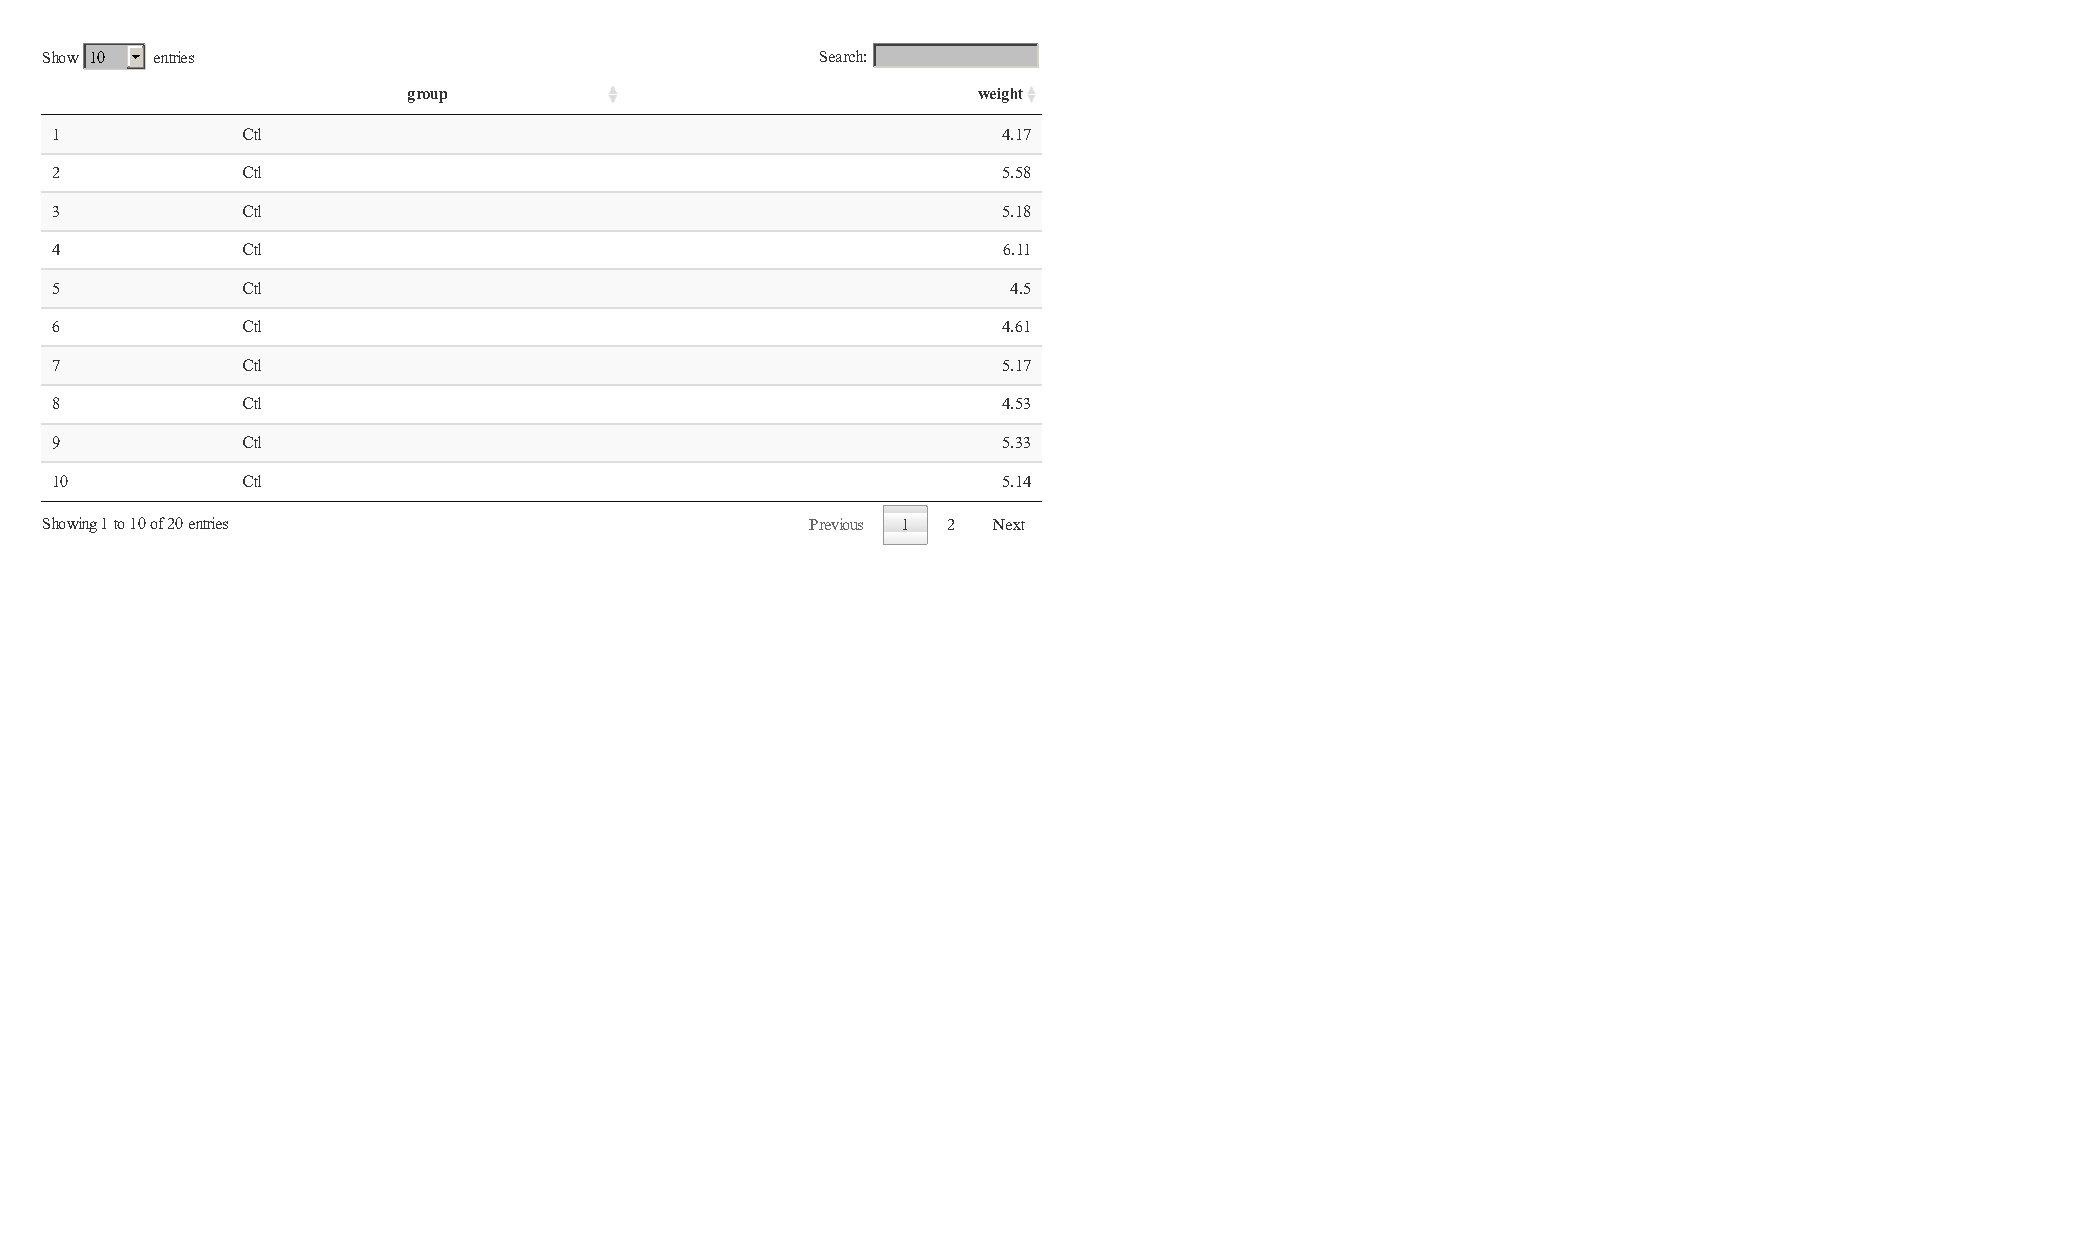
\includegraphics{SurveyBook_files/figure-latex/rawDataShow-1.pdf}

\hypertarget{visualization}{%
\subsection{Visualization}\label{visualization}}

\begin{Shaded}
\begin{Highlighting}[]
\KeywordTok{boxplot}\NormalTok{(weight}\OperatorTok{~}\StringTok{ }\NormalTok{group,}\DataTypeTok{data=}\NormalTok{Plant.Weight.Data)}
\NormalTok{weight.means <-}\StringTok{ }\KeywordTok{aggregate}\NormalTok{(weight }\OperatorTok{~}\StringTok{  }\NormalTok{group, }\DataTypeTok{data=}\NormalTok{Plant.Weight.Data, }\DataTypeTok{FUN=}\NormalTok{mean)}
\NormalTok{weight.means}
\end{Highlighting}
\end{Shaded}

\begin{verbatim}
##   group weight
## 1   Ctl  5.032
## 2   Trt  4.661
\end{verbatim}

\begin{Shaded}
\begin{Highlighting}[]
\NormalTok{weight.medians <-}\StringTok{ }\KeywordTok{aggregate}\NormalTok{(weight }\OperatorTok{~}\StringTok{  }\NormalTok{group, }\DataTypeTok{data=}\NormalTok{Plant.Weight.Data, }\DataTypeTok{FUN=}\NormalTok{median)}
\NormalTok{weight.medians}
\end{Highlighting}
\end{Shaded}

\begin{verbatim}
##   group weight
## 1   Ctl  5.155
## 2   Trt  4.550
\end{verbatim}

\begin{Shaded}
\begin{Highlighting}[]
\KeywordTok{points}\NormalTok{(}\DecValTok{1}\OperatorTok{:}\DecValTok{2}\NormalTok{, weight.means}\OperatorTok{$}\NormalTok{weight, }\DataTypeTok{pch =} \StringTok{"*"}\NormalTok{, }\DataTypeTok{col =} \StringTok{"blue"}\NormalTok{)}
\KeywordTok{text}\NormalTok{(}\KeywordTok{c}\NormalTok{(}\DecValTok{1}\OperatorTok{:}\DecValTok{2}\NormalTok{)}\OperatorTok{+}\FloatTok{0.25}\NormalTok{, weight.means}\OperatorTok{$}\NormalTok{weight, }\DataTypeTok{labels =} 
       \KeywordTok{paste}\NormalTok{(}\StringTok{"Mean = "}\NormalTok{, weight.means}\OperatorTok{$}\NormalTok{weight), }\DataTypeTok{col =} \StringTok{"blue"}\NormalTok{)}
\KeywordTok{text}\NormalTok{(}\KeywordTok{c}\NormalTok{(}\DecValTok{1}\OperatorTok{:}\DecValTok{2}\NormalTok{)}\OperatorTok{-}\FloatTok{0.25}\NormalTok{, weight.means}\OperatorTok{$}\NormalTok{weight, }\DataTypeTok{labels =} 
       \KeywordTok{paste}\NormalTok{(}\StringTok{"Median = "}\NormalTok{,weight.medians}\OperatorTok{$}\NormalTok{weight), }\DataTypeTok{col =} \StringTok{"black"}\NormalTok{)}
\end{Highlighting}
\end{Shaded}

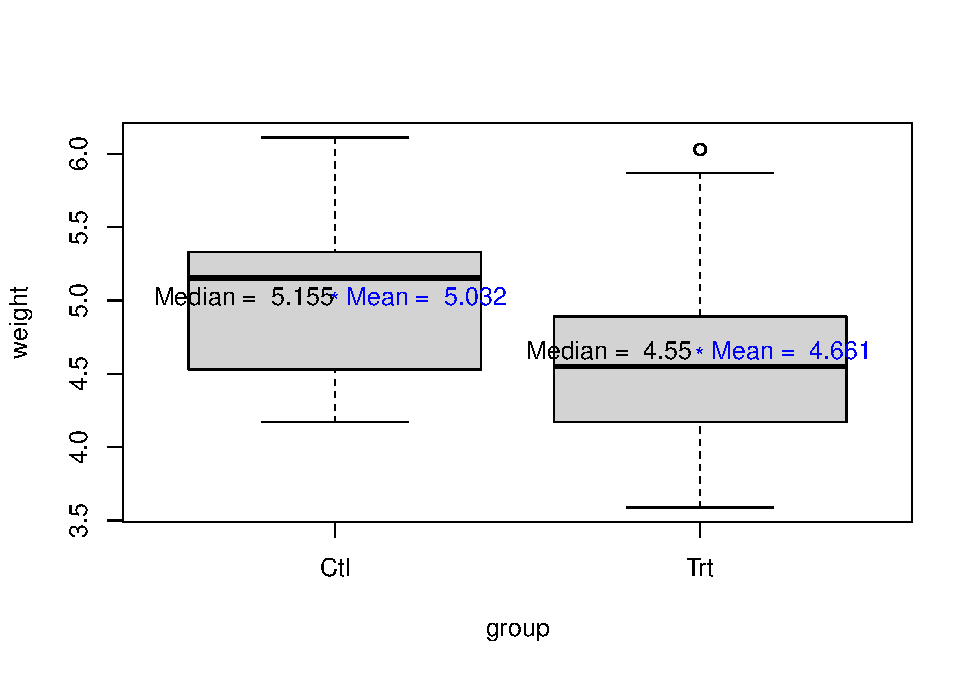
\includegraphics{SurveyBook_files/figure-latex/rawDataShow2-1.pdf}

Wait: so, plan weight reduces as we add nutrition? How confidently can we say that this added nutrition harmful for the plants (e.g., so that the weight will be reduced)?

\hypertarget{checking-assumptions}{%
\section{Checking assumptions}\label{checking-assumptions}}

Test of normality of the outcomes (Shapiro-Wilk normality test):

\begin{Shaded}
\begin{Highlighting}[]
\KeywordTok{shapiro.test}\NormalTok{(Plant.Weight.Data}\OperatorTok{$}\NormalTok{weight)}
\end{Highlighting}
\end{Shaded}

\begin{verbatim}
## 
## 	Shapiro-Wilk normality test
## 
## data:  Plant.Weight.Data$weight
## W = 0.97311, p-value = 0.8187
\end{verbatim}

Therefore, we cannot reject the null hypothesis that samples come from a population which has a normal distribution. Also check a normal quantile-quantile plot:

\begin{Shaded}
\begin{Highlighting}[]
\KeywordTok{qqnorm}\NormalTok{(Plant.Weight.Data}\OperatorTok{$}\NormalTok{weight)}
\KeywordTok{qqline}\NormalTok{(Plant.Weight.Data}\OperatorTok{$}\NormalTok{weight)}
\end{Highlighting}
\end{Shaded}

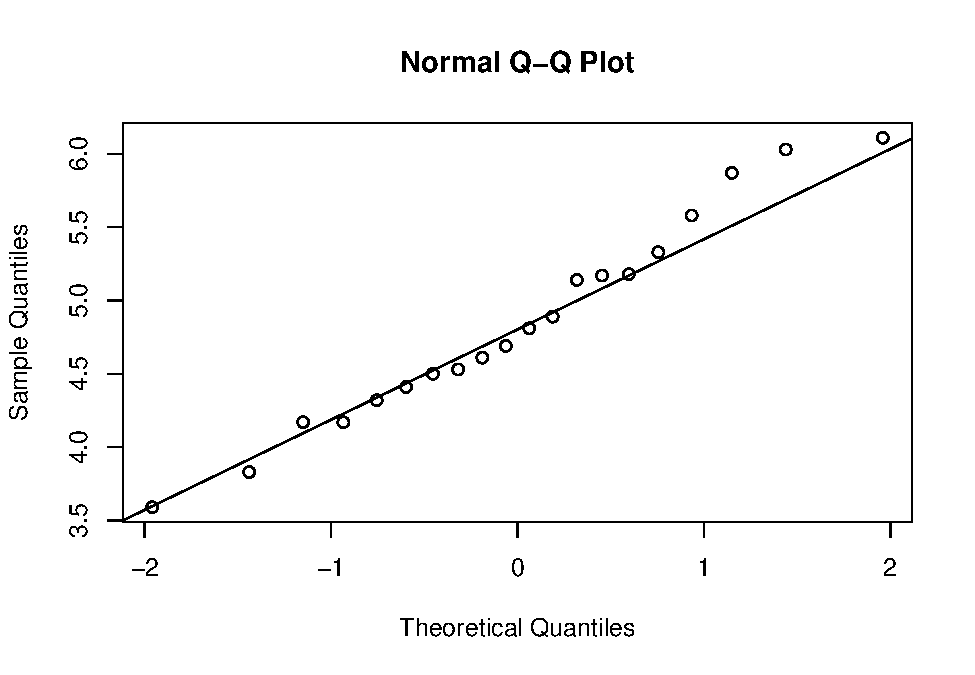
\includegraphics{SurveyBook_files/figure-latex/testing11-1.pdf}

Test of homogeneity of variances, that tests \(H_0 : \sigma_1 = \sigma_2\) vs.~\(H_1 : \sigma_1 \ne \sigma_2\):

\begin{Shaded}
\begin{Highlighting}[]
\CommentTok{# SD from each groups}
\KeywordTok{tapply}\NormalTok{(Plant.Weight.Data}\OperatorTok{$}\NormalTok{weight, }
       \DataTypeTok{INDEX =}\NormalTok{ Plant.Weight.Data}\OperatorTok{$}\NormalTok{group, }\DataTypeTok{FUN =}\NormalTok{ sd)}
\end{Highlighting}
\end{Shaded}

\begin{verbatim}
##       Ctl       Trt 
## 0.5830914 0.7936757
\end{verbatim}

\begin{Shaded}
\begin{Highlighting}[]
\KeywordTok{bartlett.test}\NormalTok{(weight }\OperatorTok{~}\StringTok{ }\NormalTok{group, }\DataTypeTok{data =}\NormalTok{ Plant.Weight.Data) }\CommentTok{# Bartlett's test}
\end{Highlighting}
\end{Shaded}

\begin{verbatim}
## 
## 	Bartlett test of homogeneity of variances
## 
## data:  weight by group
## Bartlett's K-squared = 0.79805, df = 1, p-value = 0.3717
\end{verbatim}

\begin{Shaded}
\begin{Highlighting}[]
\CommentTok{# leveneTest(weight ~ group, data = Plant.Weight.Data) # Levene's test}
\end{Highlighting}
\end{Shaded}

\hypertarget{analysis}{%
\section{Analysis}\label{analysis}}

\hypertarget{two-sample-t-test}{%
\subsection{Two-sample t-test}\label{two-sample-t-test}}

A two-sample (independent) t-test compares the weights of control and treatment group as follows (assuming equal variance; judging from the IQR from the boxplots or the above Bartlett test):

\begin{Shaded}
\begin{Highlighting}[]
\NormalTok{ttest<-}\StringTok{ }\KeywordTok{t.test}\NormalTok{(weight }\OperatorTok{~}\StringTok{ }\NormalTok{group, }\DataTypeTok{data =}\NormalTok{ Plant.Weight.Data, }
               \DataTypeTok{paired =} \OtherTok{FALSE}\NormalTok{, }\DataTypeTok{var.equal =} \OtherTok{TRUE}\NormalTok{)}
\NormalTok{ttest}
\end{Highlighting}
\end{Shaded}

\begin{verbatim}
## 
## 	Two Sample t-test
## 
## data:  weight by group
## t = 1.1913, df = 18, p-value = 0.249
## alternative hypothesis: true difference in means is not equal to 0
## 95 percent confidence interval:
##  -0.2833003  1.0253003
## sample estimates:
## mean in group Ctl mean in group Trt 
##             5.032             4.661
\end{verbatim}

Here, we test \(H_0 : \mu_1 = \mu_2 = \mu\) vs.~\(H_1 : \mu_1 \ne \mu_2\).

\begin{Shaded}
\begin{Highlighting}[]
\NormalTok{ttest}\OperatorTok{$}\NormalTok{statistic}
\end{Highlighting}
\end{Shaded}

\begin{verbatim}
##       t 
## 1.19126
\end{verbatim}

\hypertarget{regression}{%
\subsection{Regression}\label{regression}}

A simple linear model exploring the relationship between the plant weight and the group status can be fitted as follows:

\begin{Shaded}
\begin{Highlighting}[]
\NormalTok{lm.group.including.intercept <-}\StringTok{ }\KeywordTok{lm}\NormalTok{(weight }\OperatorTok{~}\StringTok{ }\DecValTok{1} \OperatorTok{+}\StringTok{ }\NormalTok{group, }\DataTypeTok{data =}\NormalTok{ Plant.Weight.Data)}
\NormalTok{lm.group.including.intercept}
\end{Highlighting}
\end{Shaded}

\begin{verbatim}
## 
## Call:
## lm(formula = weight ~ 1 + group, data = Plant.Weight.Data)
## 
## Coefficients:
## (Intercept)     groupTrt  
##       5.032       -0.371
\end{verbatim}

\begin{Shaded}
\begin{Highlighting}[]
\NormalTok{lm.group <-}\StringTok{ }\KeywordTok{lm}\NormalTok{(weight }\OperatorTok{~}\StringTok{ }\NormalTok{group, }\DataTypeTok{data =}\NormalTok{ Plant.Weight.Data)}
\NormalTok{lm.group}
\end{Highlighting}
\end{Shaded}

\begin{verbatim}
## 
## Call:
## lm(formula = weight ~ group, data = Plant.Weight.Data)
## 
## Coefficients:
## (Intercept)     groupTrt  
##       5.032       -0.371
\end{verbatim}

\begin{Shaded}
\begin{Highlighting}[]
\KeywordTok{confint}\NormalTok{(lm.group)}
\end{Highlighting}
\end{Shaded}

\begin{verbatim}
##                2.5 %    97.5 %
## (Intercept)  4.56934 5.4946602
## groupTrt    -1.02530 0.2833003
\end{verbatim}

\hypertarget{interpretation}{%
\subsubsection{Interpretation}\label{interpretation}}

Note that the variable \texttt{group} is dummy coded. \texttt{R} generally chooses the first category as the reference category.

\begin{Shaded}
\begin{Highlighting}[]
\KeywordTok{levels}\NormalTok{(}\KeywordTok{as.factor}\NormalTok{(Plant.Weight.Data}\OperatorTok{$}\NormalTok{group))}
\end{Highlighting}
\end{Shaded}

\begin{verbatim}
## [1] "Ctl" "Trt"
\end{verbatim}

\begin{enumerate}
\def\labelenumi{\arabic{enumi}.}
\tightlist
\item
  In this case, the intercept 5.032 tells us the predicted mean value for the plant weights for the control group (reference category of the group variable).
\item
  On the other hand, the slope in interpreted as the expected difference in the mean of the plant weights for that treatment group as compared to the control group. On average, weight is 0.371 units (lb?) lower in plants who are in the treatment condition compared to those in the control condition.
\end{enumerate}

\hypertarget{summary-of-the-regression-fit}{%
\subsubsection{Summary of the regression fit}\label{summary-of-the-regression-fit}}

The complete summary of the results is as follows:

\begin{Shaded}
\begin{Highlighting}[]
\KeywordTok{summary}\NormalTok{(lm.group)}
\end{Highlighting}
\end{Shaded}

\begin{verbatim}
## 
## Call:
## lm(formula = weight ~ group, data = Plant.Weight.Data)
## 
## Residuals:
##     Min      1Q  Median      3Q     Max 
## -1.0710 -0.4938  0.0685  0.2462  1.3690 
## 
## Coefficients:
##             Estimate Std. Error t value Pr(>|t|)    
## (Intercept)   5.0320     0.2202  22.850 9.55e-15 ***
## groupTrt     -0.3710     0.3114  -1.191    0.249    
## ---
## Signif. codes:  0 '***' 0.001 '**' 0.01 '*' 0.05 '.' 0.1 ' ' 1
## 
## Residual standard error: 0.6964 on 18 degrees of freedom
## Multiple R-squared:  0.07308,	Adjusted R-squared:  0.02158 
## F-statistic: 1.419 on 1 and 18 DF,  p-value: 0.249
\end{verbatim}

This is testing a different hypothesis (from the table): \(H_0: \alpha = 0\) vs.~\(H_1: \alpha \ne 0\) (\(\alpha\) being the intercept) and \(H_0: \beta = 0\) vs.~\(H_1: \beta \ne 0\) (\(\beta\) being the slope). At the bottom of the \texttt{summary} output, the \texttt{F-statistic} tests \(H_0: \beta = 0\) vs.~\(H_1: \beta \ne 0\). This is an overall, and could accomodate more slopes if the regression had more slopes. E.g., for 2 slopes, this would have tested \(H_0: \beta_1 = \beta_2 = 0\).

\hypertarget{regression-plot}{%
\subsubsection{Regression plot}\label{regression-plot}}

Let us visualize the scatter plot and the regression line:

\begin{Shaded}
\begin{Highlighting}[]
\NormalTok{Plant.Weight.Data}\OperatorTok{$}\NormalTok{group.code <-}\StringTok{ }
\StringTok{  }\KeywordTok{ifelse}\NormalTok{(Plant.Weight.Data}\OperatorTok{$}\NormalTok{group }\OperatorTok{==}\StringTok{ "Trt"}\NormalTok{, }\DecValTok{1}\NormalTok{, }\DecValTok{0}\NormalTok{)}
\NormalTok{Plant.Weight.Data}\OperatorTok{$}\NormalTok{group.code}
\end{Highlighting}
\end{Shaded}

\begin{verbatim}
##  [1] 0 0 0 0 0 0 0 0 0 0 1 1 1 1 1 1 1 1 1 1
\end{verbatim}

\begin{Shaded}
\begin{Highlighting}[]
\NormalTok{lm.code <-}\StringTok{ }\KeywordTok{lm}\NormalTok{(weight }\OperatorTok{~}\StringTok{ }\NormalTok{group.code, }\DataTypeTok{data =}\NormalTok{ Plant.Weight.Data)}
\KeywordTok{plot}\NormalTok{(weight }\OperatorTok{~}\StringTok{ }\NormalTok{group.code, }\DataTypeTok{data =}\NormalTok{ Plant.Weight.Data, }
     \DataTypeTok{axes =} \OtherTok{FALSE}\NormalTok{, }\DataTypeTok{xlab =} \StringTok{"Groups"}\NormalTok{)}
\KeywordTok{axis}\NormalTok{(}\DecValTok{1}\NormalTok{, }\DecValTok{0}\OperatorTok{:}\DecValTok{1}\NormalTok{, }\KeywordTok{levels}\NormalTok{(Plant.Weight.Data}\OperatorTok{$}\NormalTok{group))}
\KeywordTok{axis}\NormalTok{(}\DecValTok{2}\NormalTok{)}
\KeywordTok{abline}\NormalTok{(lm.code, }\DataTypeTok{col =} \StringTok{"blue"}\NormalTok{) }\CommentTok{# regression line}
\KeywordTok{abline}\NormalTok{(}\DataTypeTok{h=}\KeywordTok{coef}\NormalTok{(lm.code)[}\DecValTok{1}\NormalTok{], }\DataTypeTok{col =} \StringTok{"red"}\NormalTok{) }\CommentTok{# intercept}
\end{Highlighting}
\end{Shaded}

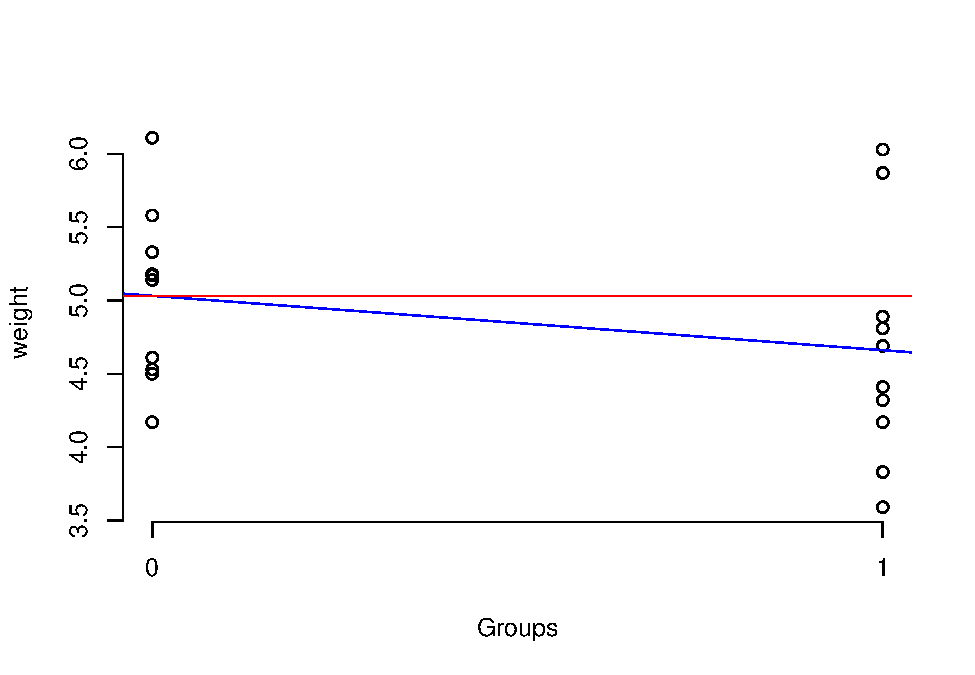
\includegraphics{SurveyBook_files/figure-latex/simpleAnalysisplot-1.pdf}

\hypertarget{assumption-checking-for-the-residuals}{%
\subsubsection{Assumption checking for the residuals}\label{assumption-checking-for-the-residuals}}

Checking normality of the residuals:

\begin{Shaded}
\begin{Highlighting}[]
\NormalTok{lm.residual <-}\StringTok{ }\KeywordTok{residuals}\NormalTok{(lm.group)}
\KeywordTok{shapiro.test}\NormalTok{(lm.residual)}
\end{Highlighting}
\end{Shaded}

\begin{verbatim}
## 
## 	Shapiro-Wilk normality test
## 
## data:  lm.residual
## W = 0.94744, p-value = 0.3299
\end{verbatim}

\begin{Shaded}
\begin{Highlighting}[]
\KeywordTok{qqnorm}\NormalTok{(lm.residual)}
\KeywordTok{qqline}\NormalTok{(lm.residual)}
\end{Highlighting}
\end{Shaded}

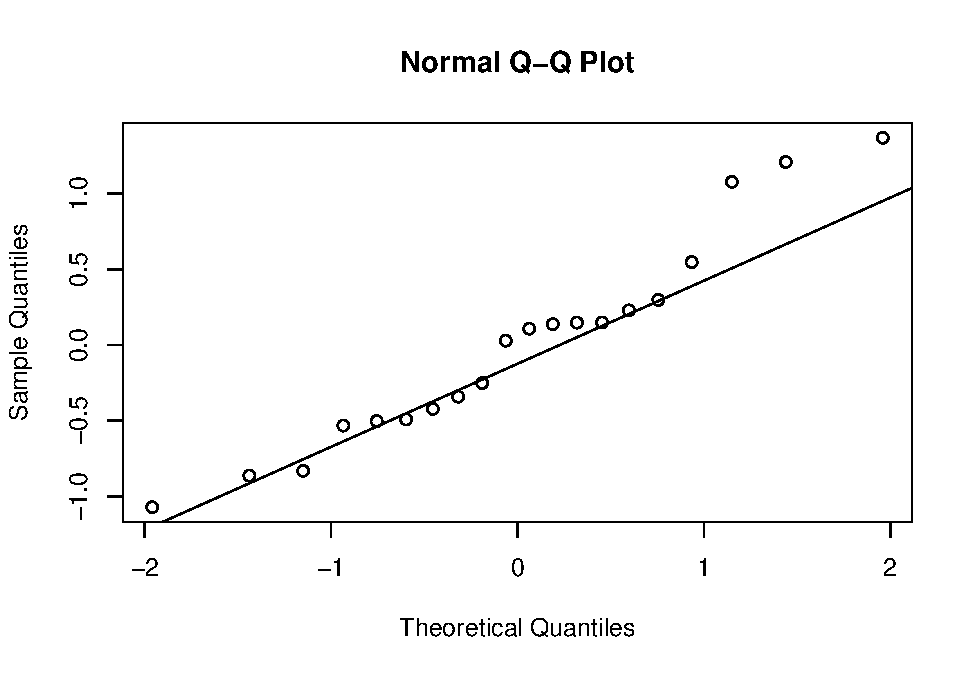
\includegraphics{SurveyBook_files/figure-latex/simpleAnalysis224-1.pdf}

\hypertarget{null-model}{%
\subsubsection{Null model}\label{null-model}}

A null model (with only intercept):

\begin{Shaded}
\begin{Highlighting}[]
\NormalTok{lm.null <-}\StringTok{ }\KeywordTok{lm}\NormalTok{(weight }\OperatorTok{~}\StringTok{ }\DecValTok{1}\NormalTok{, }\DataTypeTok{data =}\NormalTok{ Plant.Weight.Data) }\CommentTok{# Including just the intercept}
\KeywordTok{summary}\NormalTok{(lm.null)}
\end{Highlighting}
\end{Shaded}

\begin{verbatim}
## 
## Call:
## lm(formula = weight ~ 1, data = Plant.Weight.Data)
## 
## Residuals:
##     Min      1Q  Median      3Q     Max 
## -1.2565 -0.4590 -0.0965  0.3710  1.2635 
## 
## Coefficients:
##             Estimate Std. Error t value Pr(>|t|)    
## (Intercept)   4.8465     0.1574   30.79   <2e-16 ***
## ---
## Signif. codes:  0 '***' 0.001 '**' 0.01 '*' 0.05 '.' 0.1 ' ' 1
## 
## Residual standard error: 0.704 on 19 degrees of freedom
\end{verbatim}

\hypertarget{anova}{%
\subsection{ANOVA}\label{anova}}

For testing for the significance of the group membership, we can compare the current model to the null model (is adding the variable \texttt{group} in the model useful?).

\begin{Shaded}
\begin{Highlighting}[]
\KeywordTok{anova}\NormalTok{(lm.null,lm.group)}
\end{Highlighting}
\end{Shaded}

\begin{verbatim}
## Analysis of Variance Table
## 
## Model 1: weight ~ 1
## Model 2: weight ~ group
##   Res.Df    RSS Df Sum of Sq      F Pr(>F)
## 1     19 9.4175                           
## 2     18 8.7292  1   0.68821 1.4191  0.249
\end{verbatim}

Or, we could directly test \(H_0 : \mu_1 = \mu_2 = \mu\) vs.~\(H_1 : \mu_1 \ne \mu_2\) under the homogeneity of variances assumption:

\begin{Shaded}
\begin{Highlighting}[]
\KeywordTok{anova}\NormalTok{(lm.group)}
\end{Highlighting}
\end{Shaded}

\begin{verbatim}
## Analysis of Variance Table
## 
## Response: weight
##           Df Sum Sq Mean Sq F value Pr(>F)
## group      1 0.6882 0.68820  1.4191  0.249
## Residuals 18 8.7292 0.48496
\end{verbatim}

\begin{Shaded}
\begin{Highlighting}[]
\CommentTok{# Alternate ways to do the same}
\CommentTok{# car::Anova(lm.group,type="II")}
\NormalTok{aov.fit <-}\StringTok{ }\KeywordTok{aov}\NormalTok{(lm.group)}
\KeywordTok{summary}\NormalTok{(aov.fit)}
\end{Highlighting}
\end{Shaded}

\begin{verbatim}
##             Df Sum Sq Mean Sq F value Pr(>F)
## group        1  0.688  0.6882   1.419  0.249
## Residuals   18  8.729  0.4850
\end{verbatim}

\begin{Shaded}
\begin{Highlighting}[]
\CommentTok{# Multiple pairwise-comparison: }
\CommentTok{# (compare with t-test; same p-value?)}
\KeywordTok{TukeyHSD}\NormalTok{(aov.fit) }
\end{Highlighting}
\end{Shaded}

\begin{verbatim}
##   Tukey multiple comparisons of means
##     95% family-wise confidence level
## 
## Fit: aov(formula = lm.group)
## 
## $group
##           diff     lwr       upr     p adj
## Trt-Ctl -0.371 -1.0253 0.2833003 0.2490232
\end{verbatim}

Checking normality of the residuals (not run; same as above):

\begin{Shaded}
\begin{Highlighting}[]
\CommentTok{# aov.residual <- residuals(aov.fit)}
\CommentTok{# shapiro.test(aov.residual)}
\CommentTok{# qqnorm(aov.residual)}
\CommentTok{# qqline(aov.residual)}
\end{Highlighting}
\end{Shaded}

ANOVA is basically a generalization of the two-sample t-test (verify that the calculated \(F = t^2\)):

\begin{Shaded}
\begin{Highlighting}[]
\NormalTok{ttest}\OperatorTok{$}\NormalTok{statistic}\OperatorTok{^}\DecValTok{2}
\end{Highlighting}
\end{Shaded}

\begin{verbatim}
##        t 
## 1.419101
\end{verbatim}

An alternative non-parametric version of this independent 2-sample test is as follows (a Kruskal-Wallis rank sum test):

\begin{Shaded}
\begin{Highlighting}[]
\CommentTok{# Assuming groups come from similar shaped populations:}
\KeywordTok{kruskal.test}\NormalTok{(weight }\OperatorTok{~}\StringTok{ }\NormalTok{group, }\DataTypeTok{data =}\NormalTok{ Plant.Weight.Data) }
\end{Highlighting}
\end{Shaded}

\begin{verbatim}
## 
## 	Kruskal-Wallis rank sum test
## 
## data:  weight by group
## Kruskal-Wallis chi-squared = 1.7513, df = 1, p-value = 0.1857
\end{verbatim}

\hypertarget{verdict}{%
\section{Verdict}\label{verdict}}

\hypertarget{informal-conclusion}{%
\subsection{Informal conclusion}\label{informal-conclusion}}

With added nutrition, plant weights generally decrease (judging from the point estimate), but such trend could be due to sampling fluctuation (e.g., as the 95\% confidence interval includes the null value of 0) and we can not confidently (not at least with 95\% confidence) say that adding nutrition will cause plant weights to go down.

\hypertarget{a-word-of-caution}{%
\subsection{A word of caution}\label{a-word-of-caution}}

Note that, we are inherently trying to infer `causality' out of a statistical analysis, even though our hypothesis is not about `cause' explicitly. Unfortunately, correlation does not imply causation, and we need to know more about the subject-area and study-design before we make such inference or interpretation.

\hypertarget{exercises-optional}{%
\section{Exercises (Optional)}\label{exercises-optional}}

\begin{enumerate}
\def\labelenumi{\arabic{enumi}.}
\tightlist
\item
  What is the difference between a regression analysis with a dummy coded predictor variable vs.~an ANOVA?
\item
  Was multiple pairwise-comparison (\texttt{TukeyHSD}) necessary in the above example?\\
\item
  Which \texttt{R} package includes the \texttt{leveneTest} function? (hint: use \texttt{help.search()} function.)
\item
  Is `multicollinearity' an issue in the above example?
\item
  In the current example, can we interpret the slope as follows: \texttt{the\ change\ in\ Y\ for\ a\ 1-unit\ change\ in\ X} where, \(Y\) being the outcome and \(X\) being the predictor? Why, or why not?
\end{enumerate}

\hypertarget{design-based-approach}{%
\chapter{Design-based Approach}\label{design-based-approach}}

Before discussing design-based approach, let us review some of concepts related to \texttt{sampling}.

\hypertarget{sampling}{%
\section{Sampling}\label{sampling}}

\hypertarget{steps-of-generalization}{%
\subsection{Steps of generalization}\label{steps-of-generalization}}

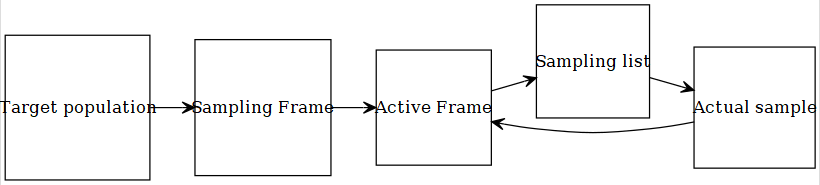
\includegraphics[width=0.65\linewidth]{images/sampling0}

Example: Let us consider CCHS.

\begin{itemize}
\tightlist
\item
  Target population: You think about a \texttt{target\ population} in you PICOT.

  \begin{itemize}
  \tightlist
  \item
    Canadian population 12 years of age and over
  \end{itemize}
\item
  Sampling Frame: But all of your target population may not belong to a \texttt{sampling\ frame} compiled by a government.

  \begin{itemize}
  \tightlist
  \item
    Canadian population 12 years of age and over exluding about 3\% population (e.g., aboriginal settlements, canadian Forces, institutionalized, foster care, 2 selected Quebec health regions)
  \end{itemize}
\item
  Active Frame: People that are still reachable

  \begin{itemize}
  \tightlist
  \item
    E.g., not dead or have not moved
  \end{itemize}
\item
  Sampling list

  \begin{itemize}
  \tightlist
  \item
    Prepared from a specific sampling technique (SRS, stratified, cluster, complex)
  \end{itemize}
\item
  Actual sample: people that have responded

  \begin{itemize}
  \tightlist
  \item
    some don't respond
  \end{itemize}
\end{itemize}

Note that, results from `actual sample' are generalized to the `active frame'. An inference from a sample may not really be generalizable to the target population (strictly speaking).

\hypertarget{types-of-sampling-techniques}{%
\subsection{Types of sampling techniques}\label{types-of-sampling-techniques}}

\begin{itemize}
\tightlist
\item
  Probability
\item
  Non-probability
\end{itemize}

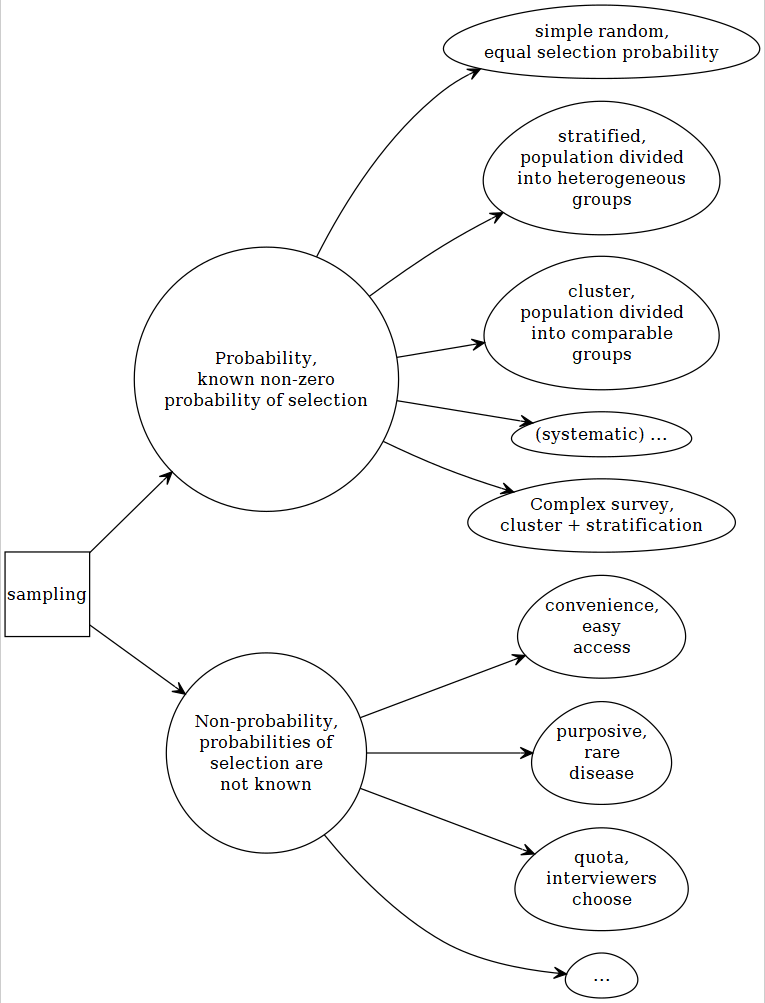
\includegraphics[width=0.85\linewidth]{images/sampling1}

\hypertarget{statistical-inference}{%
\section{Statistical inference}\label{statistical-inference}}

\hypertarget{model-based}{%
\subsection{Model-based}\label{model-based}}

Most of the statistical techniques we have seen in our pre-requisite courses (\texttt{SPPH\ 400,\ 500}) generally assumed that we are dealing with a sample that was obtained from an infinite population. We usually assume that a random process can approximate such data generation process, and the data was collected by a simple random sampling or SRS (everyone has equal opportunity to be selected in the sample). All our conclusions are based on such assumptions. If we are wrong in specifying correct distribution to approximate the data generating process, our subsequent inferences may not be valid anymore.

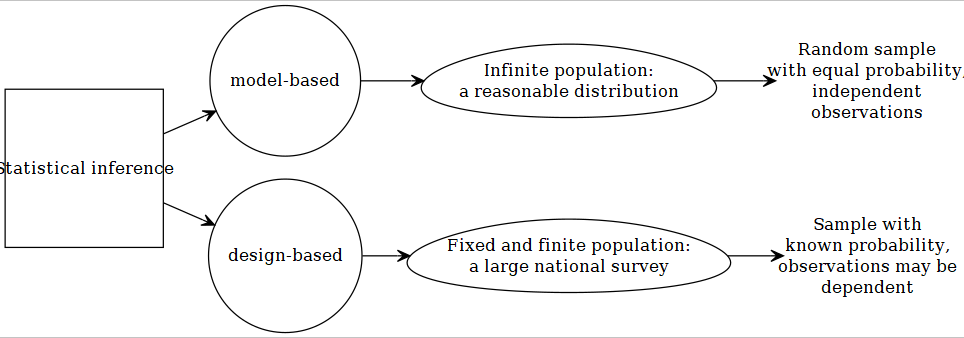
\includegraphics[width=0.85\linewidth]{images/design1}

\hypertarget{design-based}{%
\subsection{Design-based}\label{design-based}}

Generally, when wide-scale surveys are designed, simple random sampling or SRS may not be feasible for various practical considerations. May be researchers and policy-makers want that a special but small sub-group subjects should be included in our sample (e.g., people suffering from a rare disease), but it is possible that by a SRS scheme, none of the subject from that small subgroup will be included. For convenience of sampling, and for controlling variance, researchers may have to make desicions regarding how the survey needs to collect sample. Researchers may resort to cluster or stratified sampling; or a mix of both (trade-off between cost and precision). Unfortunately, in these cases, equal probability of being selected in the sample is not there any more. \citet{lumley2011complex} discussed the following properties for making design-based inference:

\begin{itemize}
\tightlist
\item
  properties needed to get valid estimates

  \begin{itemize}
  \tightlist
  \item
    non-zero probability (\(P_i>0\) for subject i) of being selected in the sample
  \item
    every subject has a known probability (\(P_i\)) of being seleted
  \end{itemize}
\item
  properties needed to acieve accuracy of those estimates

  \begin{itemize}
  \tightlist
  \item
    Every pair of subjects must have a non-zero probability (\(P_{ij}>0\) for subjects i and j) of being selected in the sample and
  \item
    that probability (\(P_{ij}\)) must be known as well.
  \end{itemize}
\end{itemize}

\hypertarget{complex-surveys}{%
\section{Complex surveys}\label{complex-surveys}}

\hypertarget{design-features}{%
\subsection{Design features}\label{design-features}}

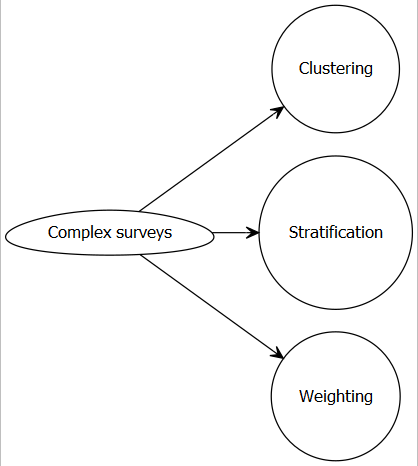
\includegraphics[width=0.45\linewidth]{images/design2}

\hypertarget{stratification}{%
\subsubsection{Stratification}\label{stratification}}

Considering sub-groups that are sufficiently different from each other with respect to characteristics. Usual examples:

\begin{itemize}
\tightlist
\item
  different geographical location: Manitoba vs.~Nunavut
\item
  high income vs.~low income
\item
  gender
\end{itemize}

For each stratum (single unit), sampling is done separately. As we can select sample size from each stratum, we are able to control for variability of the estimates (\texttt{SE}) from each strata as well.

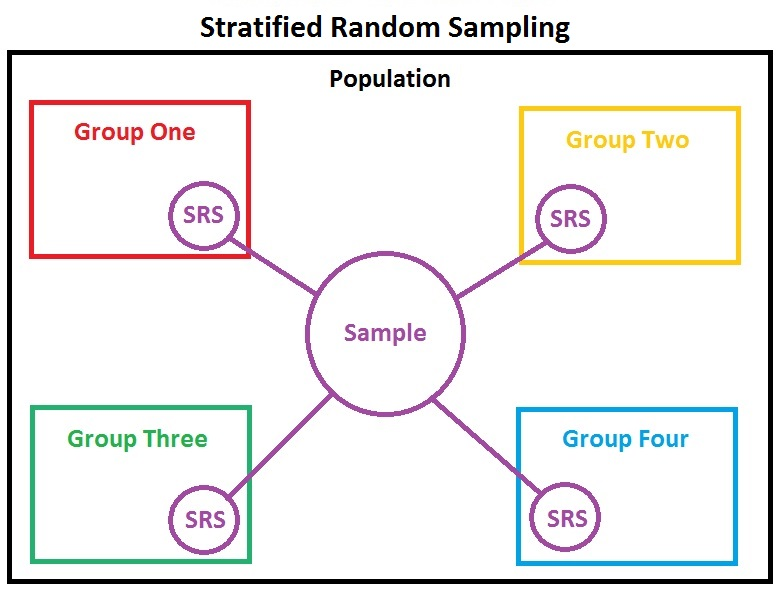
\includegraphics[width=0.85\linewidth]{images/StratifiedRandomSampling}

Source: \href{https://en.wikipedia.org/wiki/Stratified_sampling}{link}

\hypertarget{clustering}{%
\subsubsection{Clustering}\label{clustering}}

Clustering is done for convenience of data collection, generally. In a nationwide survey, researchers may choose to collect more samples from selected geographic locations. This is generally the case for cost considerations. In doing so, the surveyers don't have to travel too far, as they could essentially get many neighboring subjects at a much lower cost. An obvious consequence could be that the neighboring subjects may be more \texttt{correlated\ with\ each\ other} compared to subjects who are selected by randomness. This may cause the observations not being \texttt{independent} anymore.

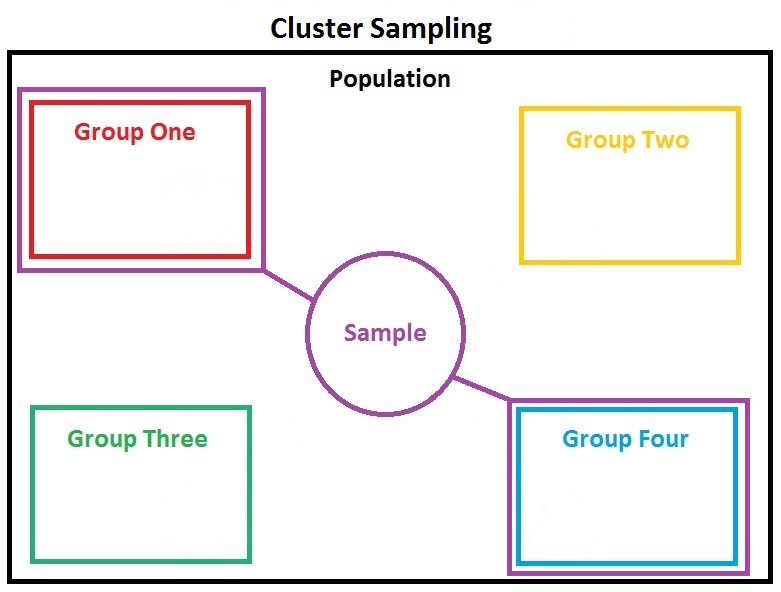
\includegraphics[width=0.85\linewidth]{images/ClusterSampling}

Source: \href{https://en.wikipedia.org/wiki/Cluster_sampling}{link}

\hypertarget{weighting}{%
\subsubsection{Weighting}\label{weighting}}

Assume that, in a SRS, a subject is selected in a sample with a probability of \(p_i = 0.04\). This mean, that person is representing \((1/p_i) = (1/0.04) = 25\) subjects in the population. We call this the \texttt{sampling\ weight} (\(w_i = 25\)). There are other type of weight:

\begin{itemize}
\tightlist
\item
  \texttt{precision\ weight}
\item
  \texttt{frequency\ weight}
\end{itemize}

but we are not really interested about those in this course in general.

In a complex survey, where we have stratification and clustering, this weight is not as straight-forward becasue, then, it is coming from an unequal probability sampling. As a consequence, not all subjects in the population will have the same probability \((p_i)\) of being included in the sample, and the sampling weights (\(w_i\)) will vary as well (but the probability or weight is known for each subjects).

\hypertarget{design-effect}{%
\subsection{Design effect}\label{design-effect}}

Compared to a SRS, all of the design features of a complex survey, such as, stratification, cluster sampling, and weighting generally influence the SEs of the estimates. Survey researchers use a ratio called design effect, to account for the difference in SEs between a complex survey versus a SRS:

\(DE^2 = \frac{SE^2_{Complex.Survey}}{SE^2_{SRS}}\).

\hypertarget{other-ideas}{%
\section{Other ideas}\label{other-ideas}}

\begin{itemize}
\tightlist
\item
  \href{https://wwwn.cdc.gov/nchs/nhanes/tutorials/module2.aspx}{Oversampling}
\end{itemize}

\hypertarget{further-readings}{%
\section{Further readings}\label{further-readings}}

Available via UBC library:

\begin{itemize}
\tightlist
\item
  Chapter 2 of \citet{heeringa2017applied}
\item
  Chapter 1 of \citet{lumley2011complex}
\item
  Section 6.3 of \citet{bilder2014analysis}
\item
  Chapter 12 of \citet{vittinghoff2011regression}
\end{itemize}

\hypertarget{exercise}{%
\section{Exercise}\label{exercise}}

\begin{itemize}
\tightlist
\item
  Skim through the first chapter (from the further readings list). Should be easier to read most of it after this lecture.
\item
  If any terminology remains unfamiliar, please discuss on Canvas.
\end{itemize}

\hypertarget{potential-data-sources}{%
\chapter{Potential Data Sources}\label{potential-data-sources}}

\hypertarget{survey-data-with-features}{%
\section{Survey data with features}\label{survey-data-with-features}}

\begin{itemize}
\tightlist
\item
  Canadian Community Health Survey - Annual Component \href{https://www150.statcan.gc.ca/n1/en/catalogue/11-625-X}{CCHS}

  \begin{itemize}
  \tightlist
  \item
    Download link \href{http://dvn.library.ubc.ca/}{UBC library}
  \end{itemize}
\item
  National Health and Nutrition Examination Survey \href{https://www.cdc.gov/nchs/nhanes/index.htm}{NHANES}

  \begin{itemize}
  \tightlist
  \item
    R packages to download data: \href{https://cran.r-project.org/web/packages/nhanesA/vignettes/Introducing_nhanesA.html}{nhanesA}, \href{https://cran.r-project.org/web/packages/RNHANES/vignettes/introduction.html}{RNHANES}
  \end{itemize}
\item
  National Longitudinal Study of Adolescent to Adult Health {[}Add Health{]}, 1994-2008 \href{http://www.icpsr.umich.edu/icpsrweb/DSDR/studies/21600}{ICPSR 21600}
\item
  European Social Survey \href{http://www.europeansocialsurvey.org/}{ESS}

  \begin{itemize}
  \tightlist
  \item
    R package to download data: \href{https://cran.r-project.org/web/packages/essurvey/vignettes/intro_ess.html}{essurvey}
  \end{itemize}
\item
  Behavioral Risk Factor Surveillance System \href{https://www.cdc.gov/brfss/data_documentation/index.htm}{BRFSS}
\item
  Bureau of Economic Analysis \href{http://www.bea.gov/}{BEA}
\item
  US National Vital Statistics System \href{https://www.cdc.gov/nchs/nvss/vsrr.htm}{NVSS}
\end{itemize}

\hypertarget{others}{%
\section{Others}\label{others}}

\begin{itemize}
\tightlist
\item
  Vanderbilt Biostatistics Datasets \href{http://biostat.mc.vanderbilt.edu/wiki/Main/DataSets}{link}
\item
  World Bank Open Data \href{https://data.worldbank.org/}{WBOD}

  \begin{itemize}
  \tightlist
  \item
    R packages to download data: \href{https://cran.r-project.org/web/packages/wbstats/vignettes/Using_the_wbstats_package.html}{wbstats}, \href{https://cran.r-project.org/web/packages/WDI/index.html}{WDI}
  \end{itemize}
\end{itemize}

\hypertarget{importing-cchs-to-r}{%
\chapter{Importing CCHS to R}\label{importing-cchs-to-r}}

This is a short instruction document of how to get CCHS dataset from the UBC library site to your RStudio environment. Once we bring the dataset into RStudio, the next step is to think about creating analytic dataset.

\hypertarget{downloading-cchs-data-from-ubc}{%
\section{Downloading CCHS data from UBC}\label{downloading-cchs-data-from-ubc}}

\begin{itemize}
\tightlist
\item
  \textbf{Step 1}: Go to \href{http://dvn.library.ubc.ca}{dvn.library.ubc.ca}, and press `log-in'
\end{itemize}

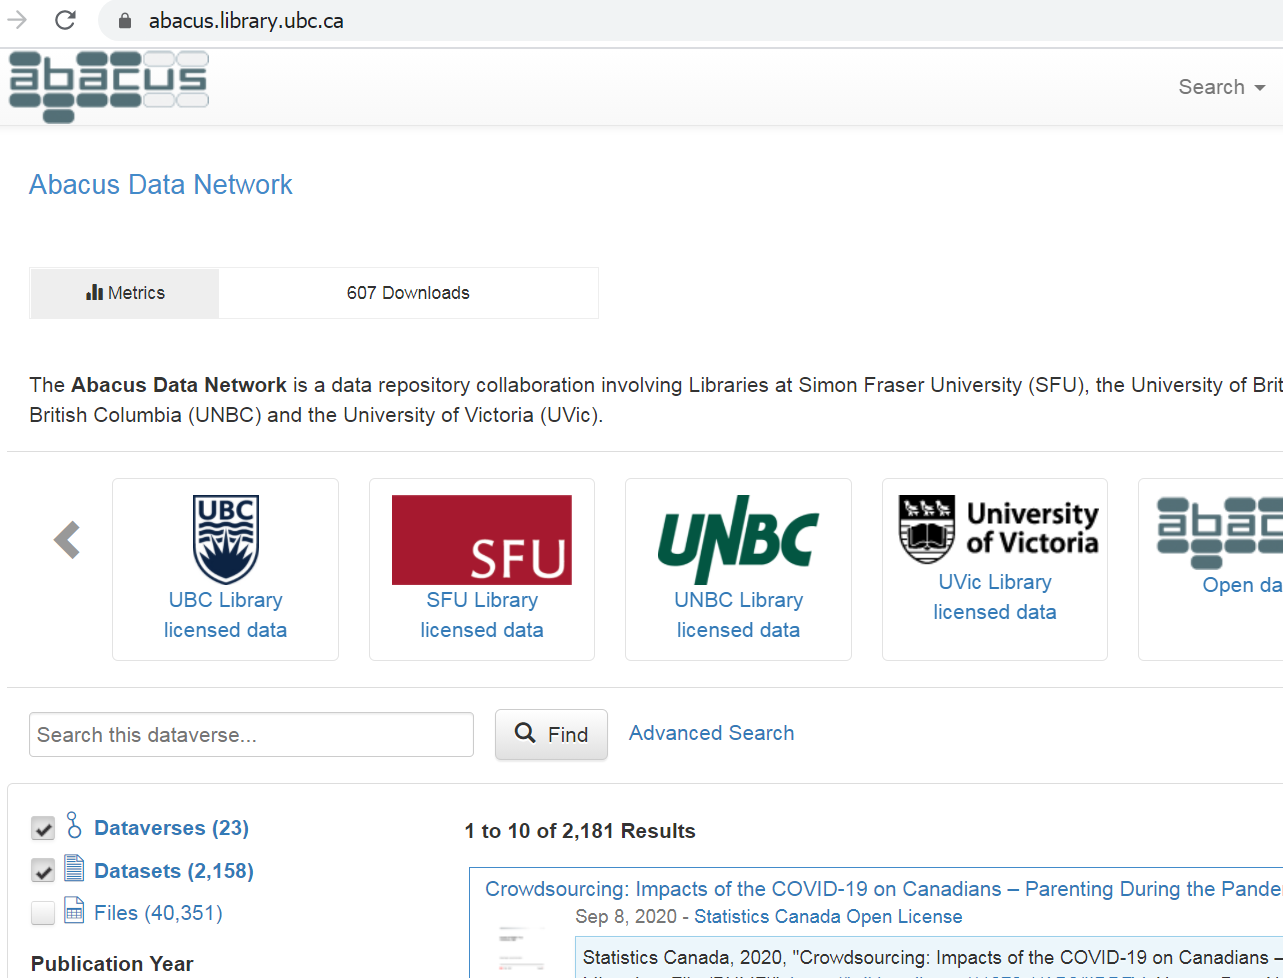
\includegraphics[width=0.65\linewidth]{images/abacusX1}

\begin{itemize}
\tightlist
\item
  \textbf{Step 2}: Select `UBC' from the dropdown menu
\end{itemize}

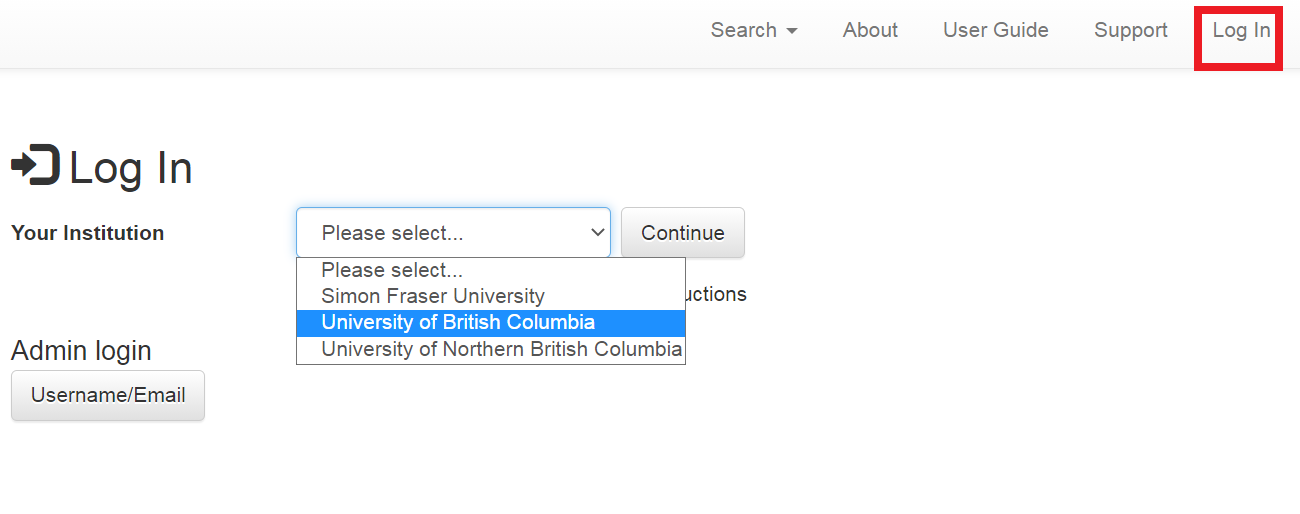
\includegraphics[width=0.65\linewidth]{images/abacusX2}

\begin{itemize}
\tightlist
\item
  \textbf{Step 3}: Enter your CWL or UBC library authentication information
\end{itemize}

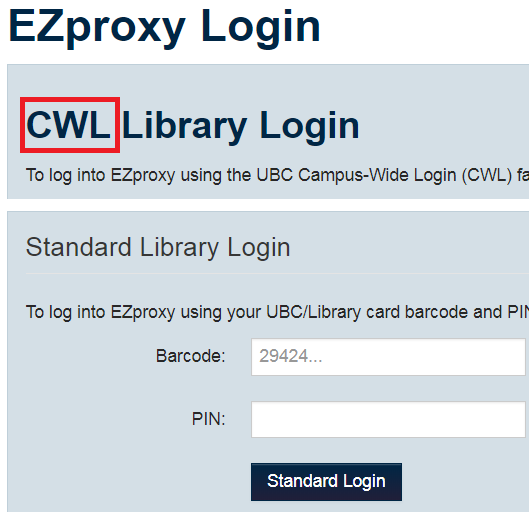
\includegraphics[width=0.65\linewidth]{images/abacus3}

\begin{itemize}
\tightlist
\item
  \textbf{Step 4}: Once you log-in, search the term `cchs' in the search-box
\end{itemize}

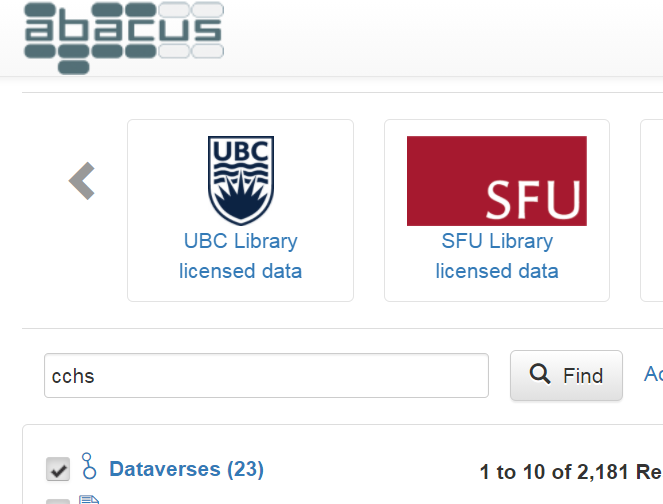
\includegraphics[width=0.65\linewidth]{images/abacusX4}

\begin{itemize}
\tightlist
\item
  \textbf{Step 5}: For illustrative purposes, let us work with the Cycle 3.1 of the CCHS dataset from the list of results. In that case, type `cchs 3.1'
\end{itemize}

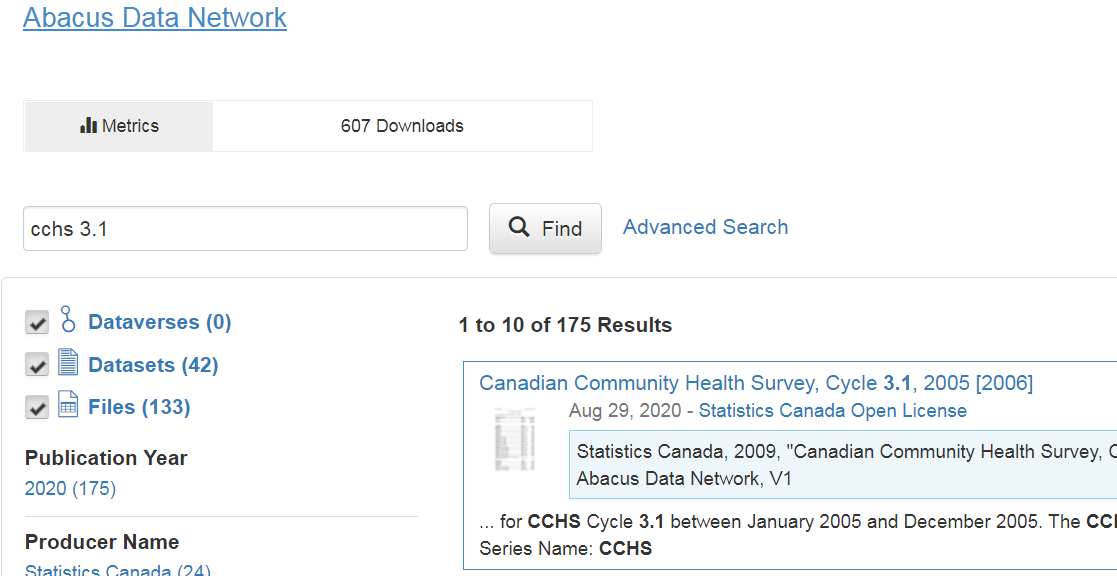
\includegraphics[width=0.65\linewidth]{images/abacusX5}

\begin{itemize}
\tightlist
\item
  \textbf{Step 6}: CCHS Cycle 3.1 information
\end{itemize}

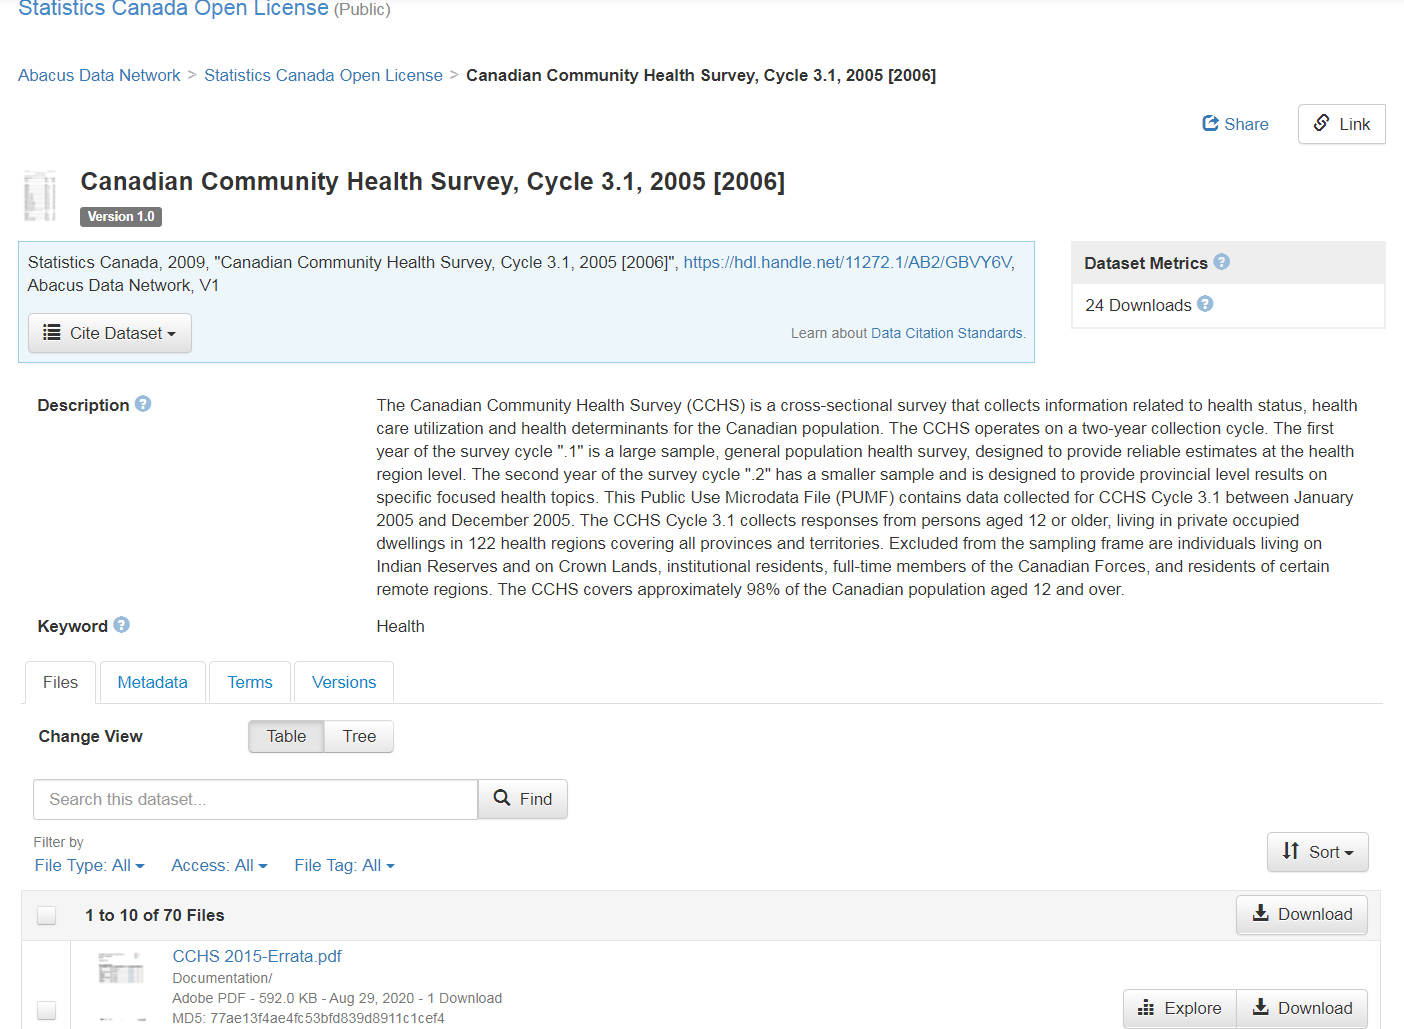
\includegraphics[width=0.65\linewidth]{images/abacus6X}

\begin{itemize}
\tightlist
\item
  \textbf{Step 7}: Choose the `Data: CD' from the menu
\end{itemize}

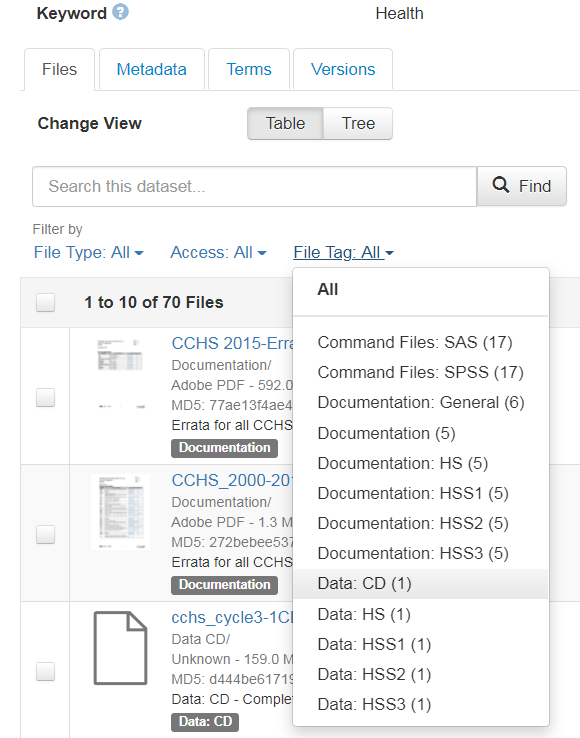
\includegraphics[width=0.65\linewidth]{images/abacusX7}

\begin{itemize}
\tightlist
\item
  \textbf{Step 8}: Download the entire data (about 159 MB) as a zip file
\end{itemize}

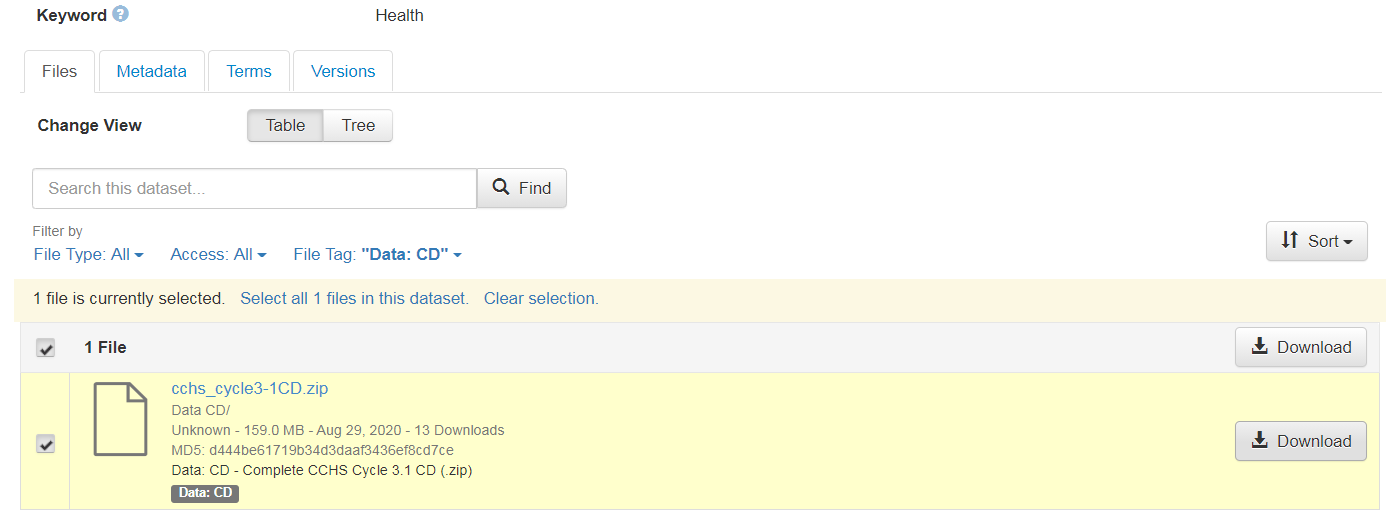
\includegraphics[width=0.65\linewidth]{images/abacusX8}

\begin{itemize}
\tightlist
\item
  \textbf{Step 9}: Accept the `terms of use'
\end{itemize}

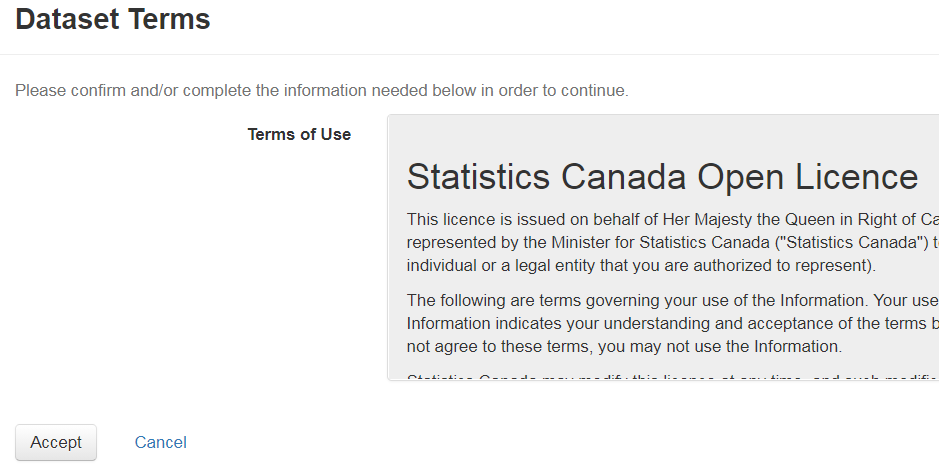
\includegraphics[width=0.65\linewidth]{images/abacusX9}

\begin{itemize}
\tightlist
\item
  \textbf{Step 10}: Select a directory to download the zip file. The path of the download directory is important (we need to use this \texttt{path} exactly later). For example, below we are in \texttt{"C:\textbackslash{}CCHS\textbackslash{}"} folder, but we will create a ``Data'' folder there, so that the download path is \texttt{"C:\textbackslash{}CCHS\textbackslash{}Data\textbackslash{}"}.
\end{itemize}

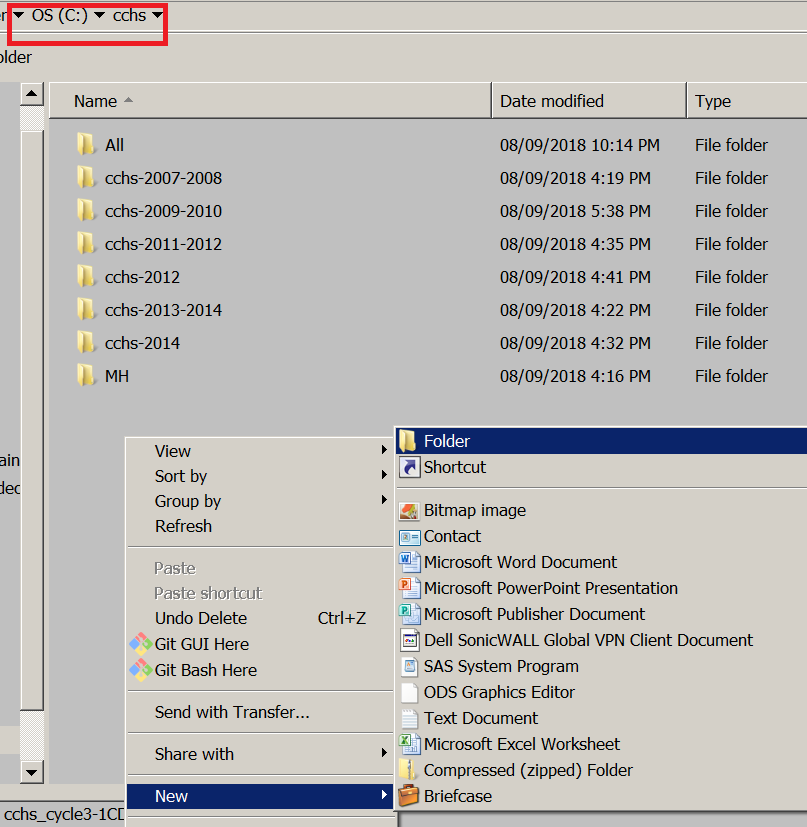
\includegraphics[width=0.65\linewidth]{images/abacusX10}

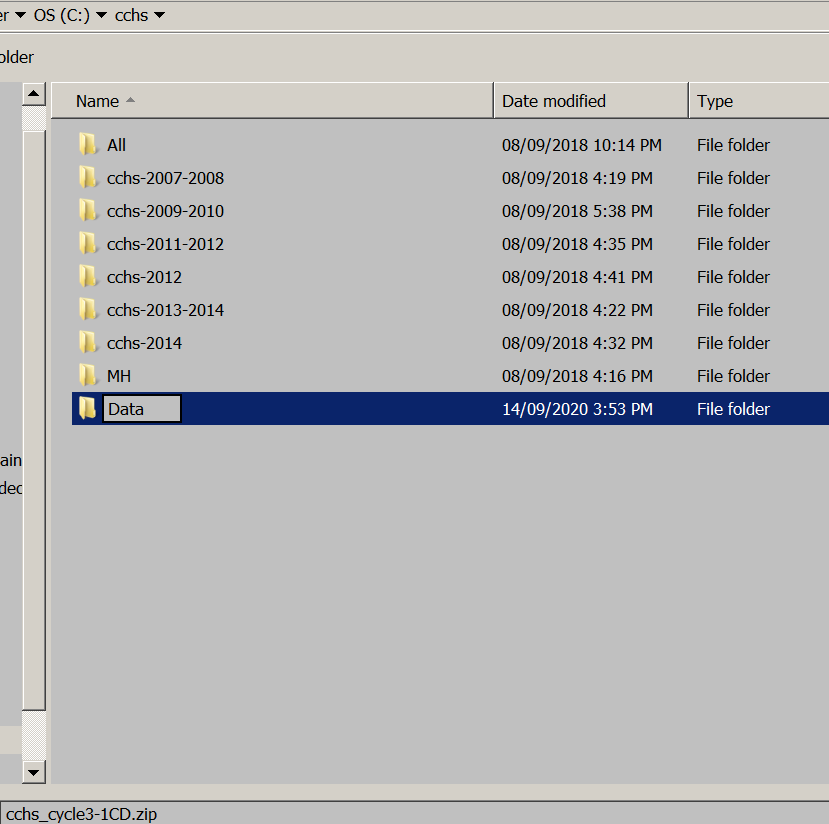
\includegraphics[width=0.65\linewidth]{images/abacusX10b}

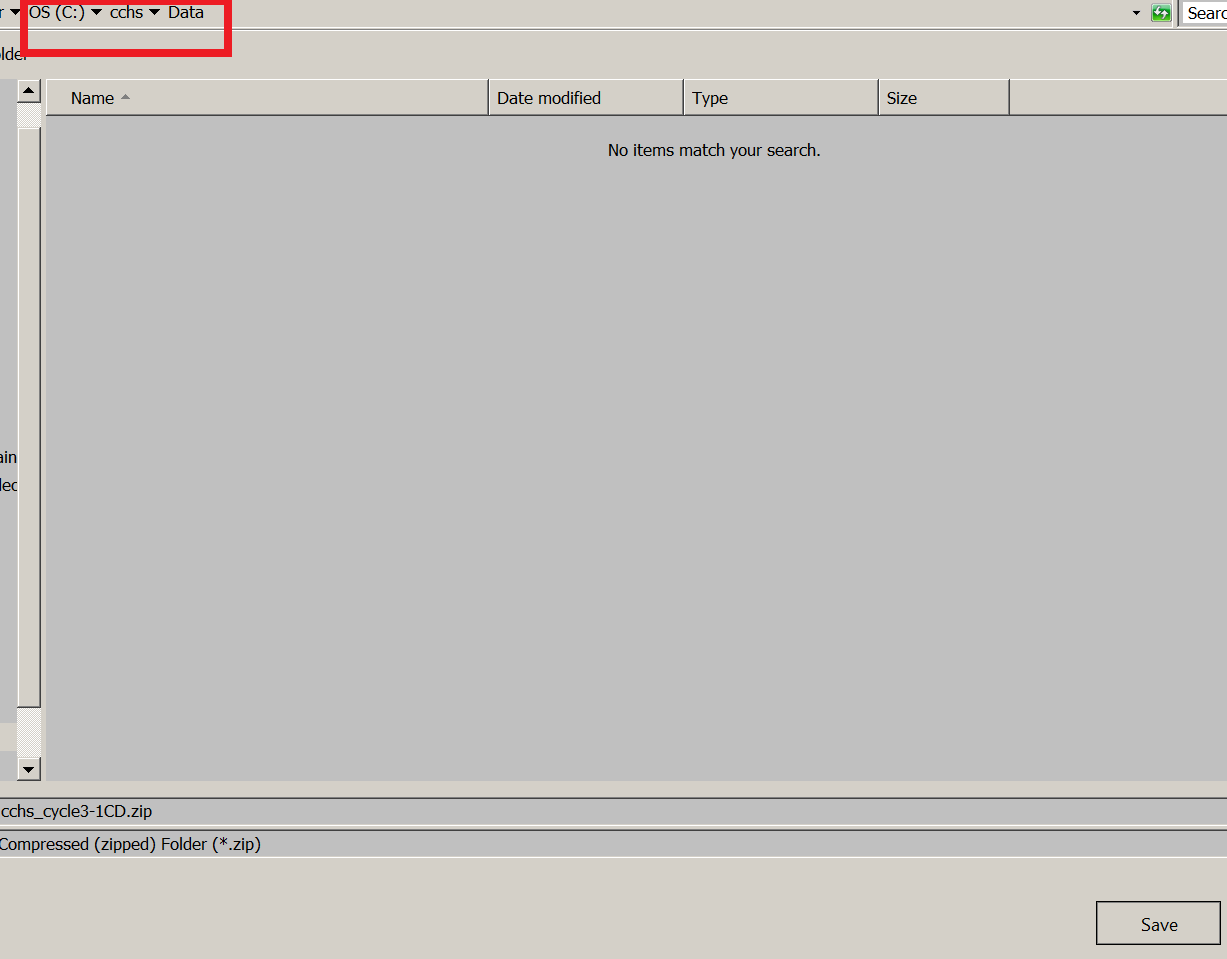
\includegraphics[width=0.65\linewidth]{images/abacusX10c}

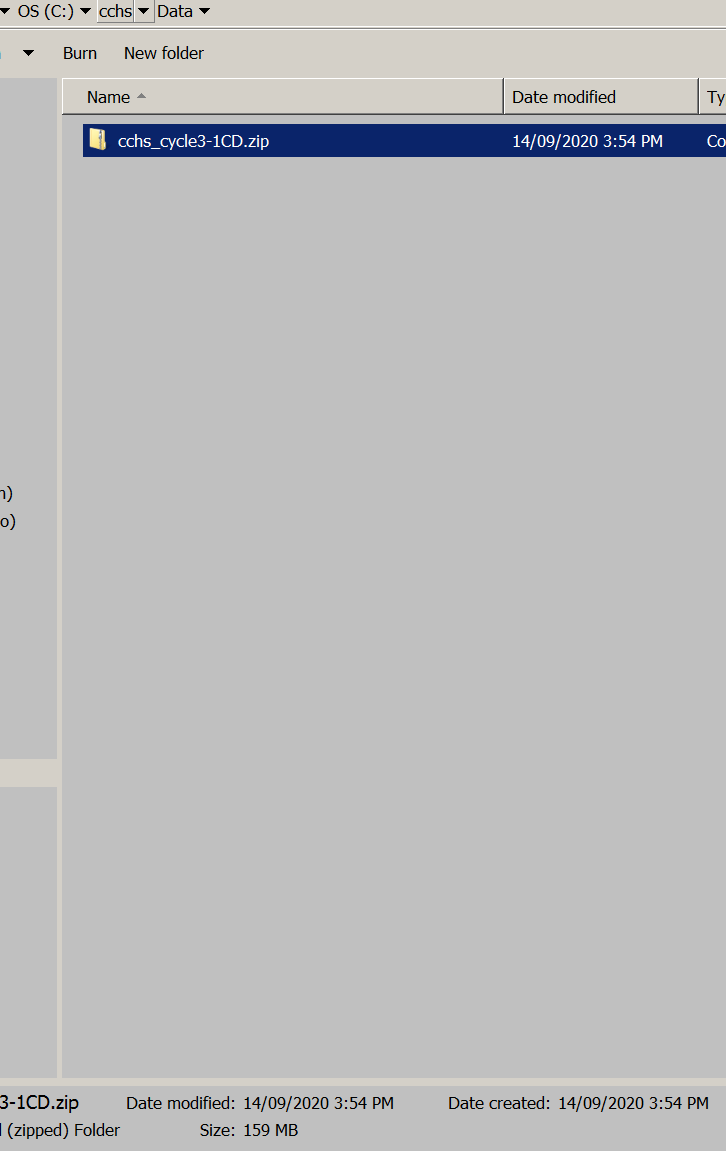
\includegraphics[width=0.65\linewidth]{images/abacusX10d}

\begin{itemize}
\tightlist
\item
  \textbf{Step 11}: Extract the zip file
\end{itemize}

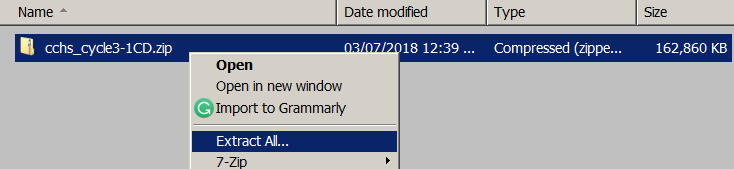
\includegraphics[width=0.65\linewidth]{images/abacus11}

\begin{itemize}
\tightlist
\item
  \textbf{Step 12}: Be patient with the extraction
\end{itemize}

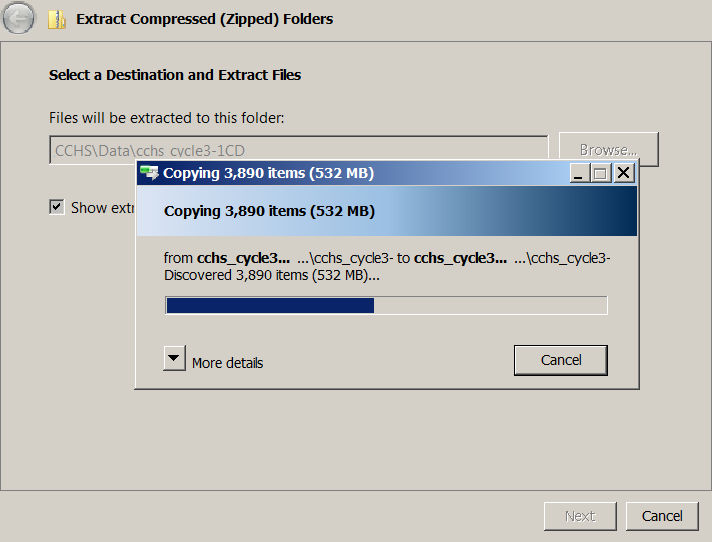
\includegraphics[width=0.65\linewidth]{images/abacus12}

\begin{itemize}
\tightlist
\item
  \textbf{Step 13}: Once extraction is complete, take a look at the folders inside. You will see that there is a folder named `SAS\_SPSS'
\end{itemize}

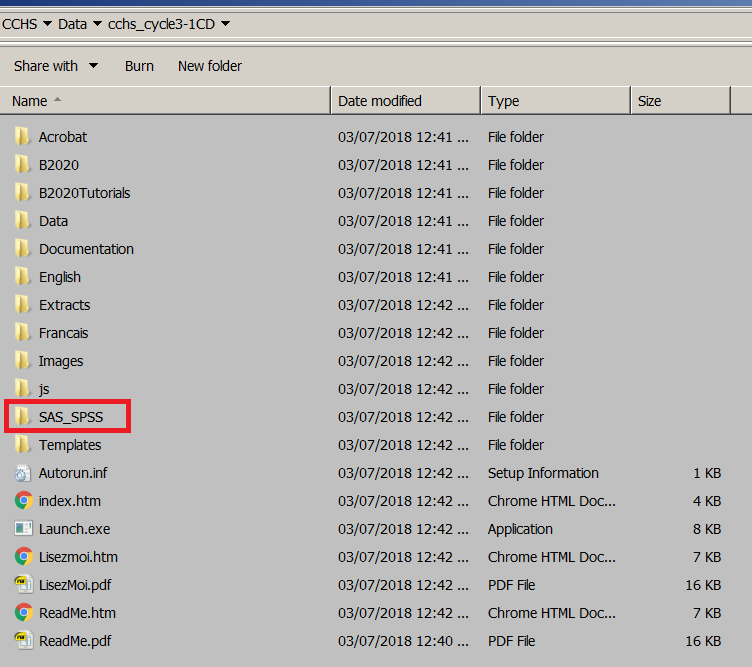
\includegraphics[width=0.65\linewidth]{images/abacus13}

\hypertarget{reading-and-formatting-the-data}{%
\section{Reading and Formatting the data}\label{reading-and-formatting-the-data}}

\hypertarget{option-1-processing-data-using-sas}{%
\subsection{Option 1: Processing data using SAS}\label{option-1-processing-data-using-sas}}

SAS is a commercial software. You may be able to get access to educational version. In case you don't have access to it, later we outline how to use free packages to read these datasets.

\begin{itemize}
\tightlist
\item
  \textbf{Step 1}: Inside that `SAS\_SPSS' folder, find the file \emph{hs\_pfe.sas}. It is a long file, but we are going to work on part of it. First thing we want to do it to change all the directory names to where you have unzipped the downloaded file (for example, here the zip file was extracted to C:/CCHS/Data/cchs\_cycle3-1CD/). We only need the first part of the code (as shown below; only related to data `hs'). Delete the rest of the codes for now. The resulting code should like like this:
\end{itemize}

\begin{Shaded}
\begin{Highlighting}[]
\NormalTok{%include }\StringTok{"C:\textbackslash{}CCHS\textbackslash{}Data\textbackslash{}cchs_cycle3-1CD\textbackslash{}SAS_SPSS\textbackslash{}Layouts\textbackslash{}hs\textbackslash{}hs_pfe.sas"}\NormalTok{;}

\NormalTok{data hs;}
\NormalTok{        %let datafid=}\StringTok{"C:\textbackslash{}CCHS\textbackslash{}Data\textbackslash{}cchs_cycle3-1CD\textbackslash{}Data\textbackslash{}hs.txt"}\NormalTok{;}
\NormalTok{		%include }\StringTok{"C:\textbackslash{}CCHS\textbackslash{}Data\textbackslash{}cchs_cycle3-1CD\textbackslash{}SAS_SPSS\textbackslash{}Layouts\textbackslash{}hs\textbackslash{}hs_i.sas"}\NormalTok{;}
\NormalTok{        %include }\StringTok{"C:\textbackslash{}CCHS\textbackslash{}Data\textbackslash{}cchs_cycle3-1CD\textbackslash{}SAS_SPSS\textbackslash{}Layouts\textbackslash{}hs\textbackslash{}hs_fmt.sas"}\NormalTok{;}
\NormalTok{        %include }\StringTok{"C:\textbackslash{}CCHS\textbackslash{}Data\textbackslash{}cchs_cycle3-1CD\textbackslash{}SAS_SPSS\textbackslash{}Layouts\textbackslash{}hs\textbackslash{}hs_lbe.sas"}\NormalTok{;}
\NormalTok{run;}
\end{Highlighting}
\end{Shaded}

Once the modifications are done, submit the codes in SAS. Note that, the name of the data is `hs'.

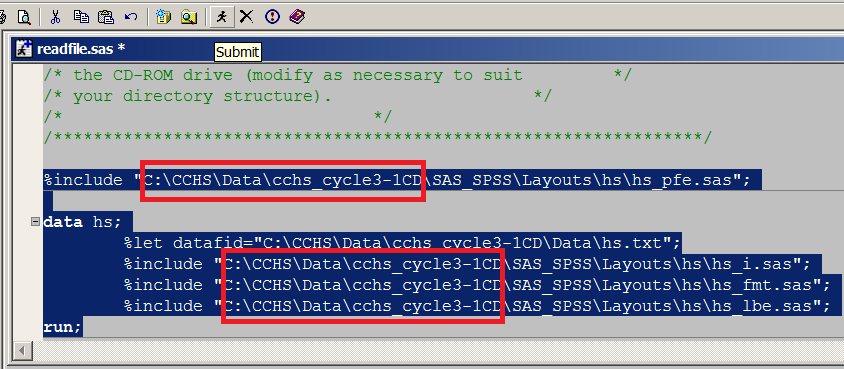
\includegraphics[width=0.65\linewidth]{images/abacus14}

\begin{itemize}
\tightlist
\item
  \textbf{Step 2}: Once you submit the code, you can check the log window in SAS to see how the code submission went. It should tell you how many observations and variables were read.
\end{itemize}

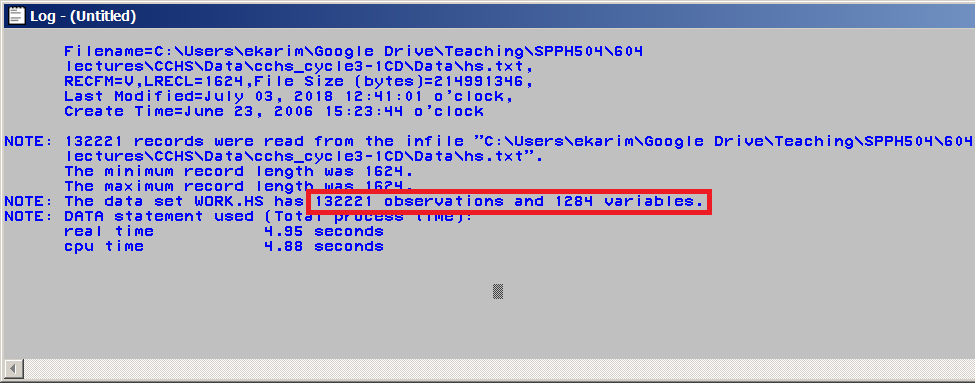
\includegraphics[width=0.65\linewidth]{images/abacus15}

\begin{itemize}
\tightlist
\item
  \textbf{Step 3}: If you one to view the dataset, you can go to `Explorer' window within SAS.
\end{itemize}

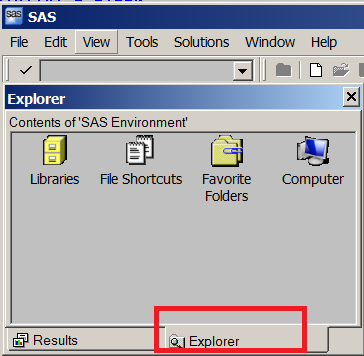
\includegraphics[width=0.65\linewidth]{images/abacus16}

\begin{itemize}
\tightlist
\item
  \textbf{Step 4}: Generally, if you haven't specified where to load the files, SAS will by default save the data into a library called `Work'
\end{itemize}

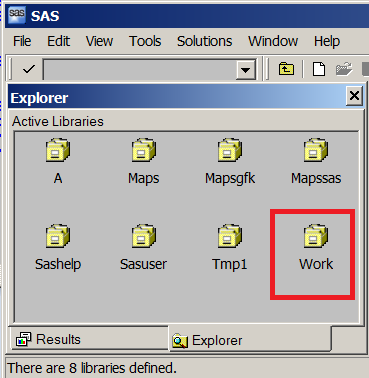
\includegraphics[width=0.65\linewidth]{images/abacus17}

\begin{itemize}
\tightlist
\item
  \textbf{Step 5}: Open that folder, and you will be able to find the dataset `Hs'.
\end{itemize}

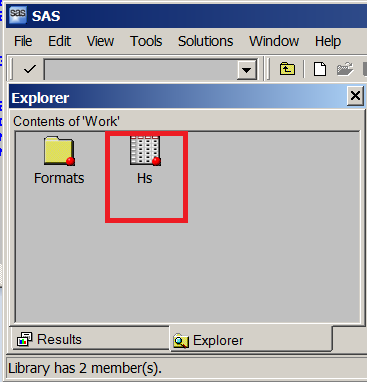
\includegraphics[width=0.65\linewidth]{images/abacus18}

\begin{itemize}
\tightlist
\item
  \textbf{Step 6}: Right click on the data, and click `open' to view the datafile.
\end{itemize}

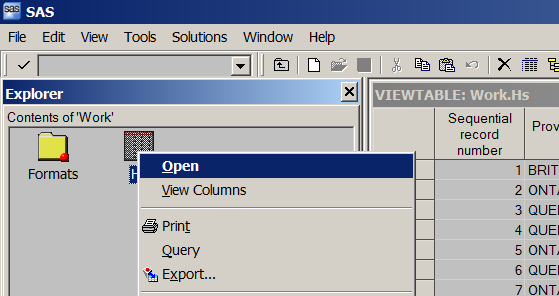
\includegraphics[width=0.65\linewidth]{images/abacus19}

\begin{itemize}
\tightlist
\item
  \textbf{Step 7}: To export the data into a CSV format data (so that we can read this data into other software packages), ckick `Menu'.
\end{itemize}

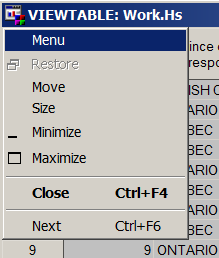
\includegraphics[width=0.65\linewidth]{images/abacus20}

\begin{itemize}
\tightlist
\item
  \textbf{Step 8}: then press `Export Data'.
\end{itemize}

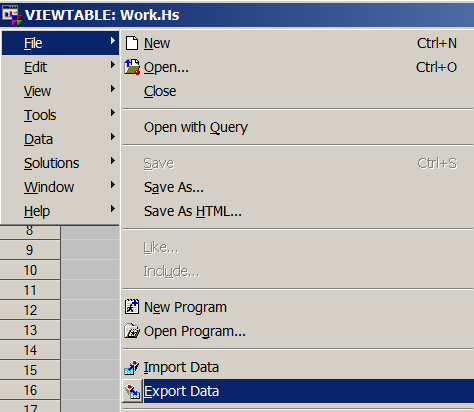
\includegraphics[width=0.65\linewidth]{images/abacus21}

\begin{itemize}
\tightlist
\item
  \textbf{Step 9}: choose the library and the data.
\end{itemize}

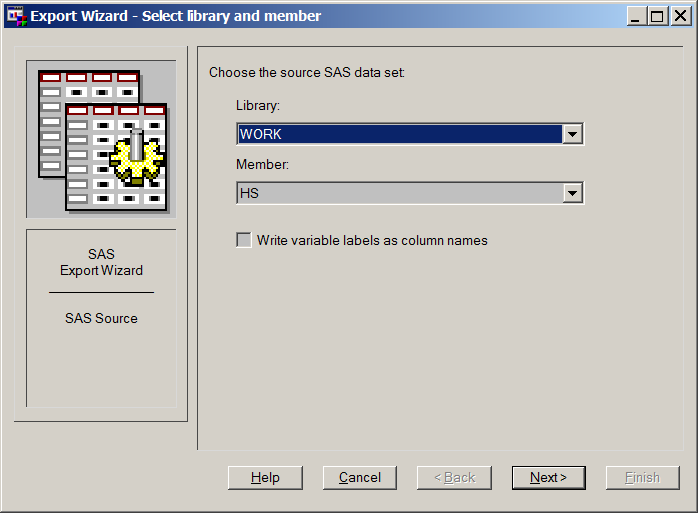
\includegraphics[width=0.65\linewidth]{images/abacus22}

\begin{itemize}
\tightlist
\item
  \textbf{Step 10}: choose the format in which you may want to save the existing data.
\end{itemize}

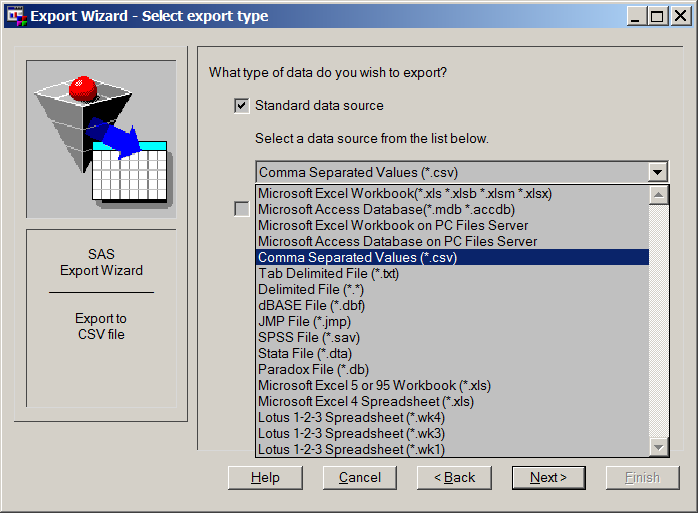
\includegraphics[width=0.65\linewidth]{images/abacus23}

\begin{itemize}
\tightlist
\item
  \textbf{Step 11}: also specify where you want to save the csv file and the name of that file (e.g., cchs3.csv).
\end{itemize}

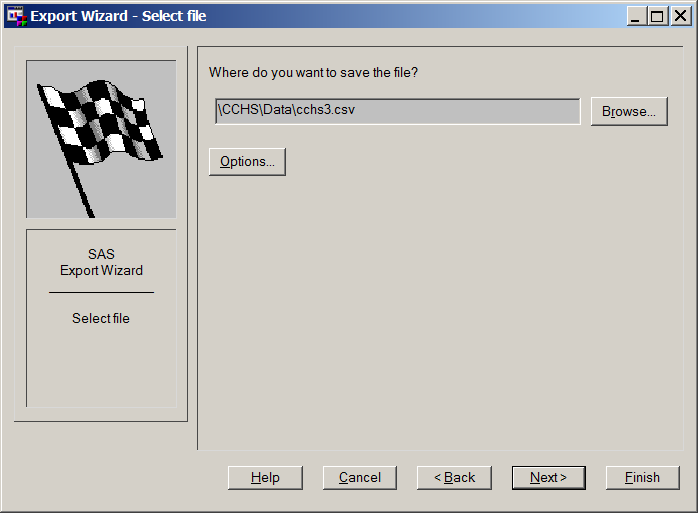
\includegraphics[width=0.65\linewidth]{images/abacus24}

\begin{itemize}
\tightlist
\item
  \textbf{Step 12}: go to that directory to see the file cchs3.csv
\end{itemize}

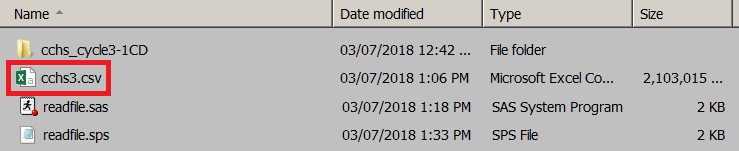
\includegraphics[width=0.65\linewidth]{images/abacus25}

\begin{itemize}
\tightlist
\item
  \textbf{Step 13}: If you want to save the file in SAS format, you can do so by writing the following sas code into the `Editor' window. Here we are saving the data Hs within the Work library in to a data called cchs3 within the SASLib library. Note that, the directory name has to be where you want to save the output file.
\end{itemize}

\begin{Shaded}
\begin{Highlighting}[]
\NormalTok{LIBNAME SASLib }\StringTok{"C:\textbackslash{}CCHS\textbackslash{}Data"}\NormalTok{;}
\NormalTok{DATA SASLib.cchs3;}
\NormalTok{    set Work.Hs;}
\NormalTok{run;}
\end{Highlighting}
\end{Shaded}

Submit these codes into SAS:

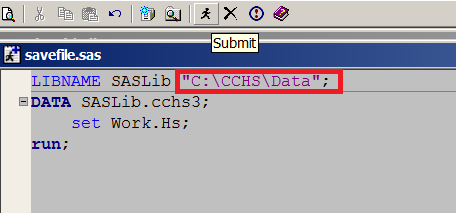
\includegraphics[width=0.65\linewidth]{images/abacus26}

\begin{itemize}
\tightlist
\item
  \textbf{Step 13}: go to that directory to see the file cchs3.sas7dbat
\end{itemize}

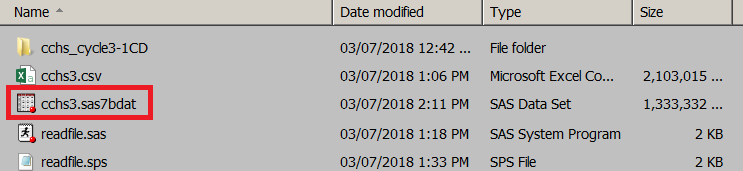
\includegraphics[width=0.65\linewidth]{images/abacus27}

\hypertarget{option-2-processing-data-using-pspp-free}{%
\subsection{Option 2: Processing data using PSPP (Free)}\label{option-2-processing-data-using-pspp-free}}

PSPP is a free package; alternative to commercial software SPSS. We can use the same SPSS codes to read the datafile into PSPP, and save.

\begin{itemize}
\tightlist
\item
  \textbf{Step 1}: Get the free PSPP software from the website: \href{http://www.gnu.org/software/pspp/}{www.gnu.org/software/pspp/}
\end{itemize}

PSPP is available for GNU/Hurd, GNU/Linux, Darwin (Mac OS X), OpenBSD, NetBSD, FreeBSD, and Windows

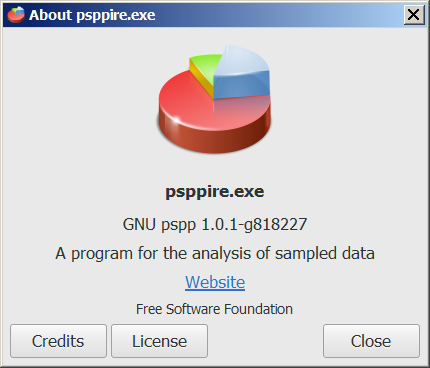
\includegraphics[width=0.65\linewidth]{images/abacus30}

For windows, download appropriate version.

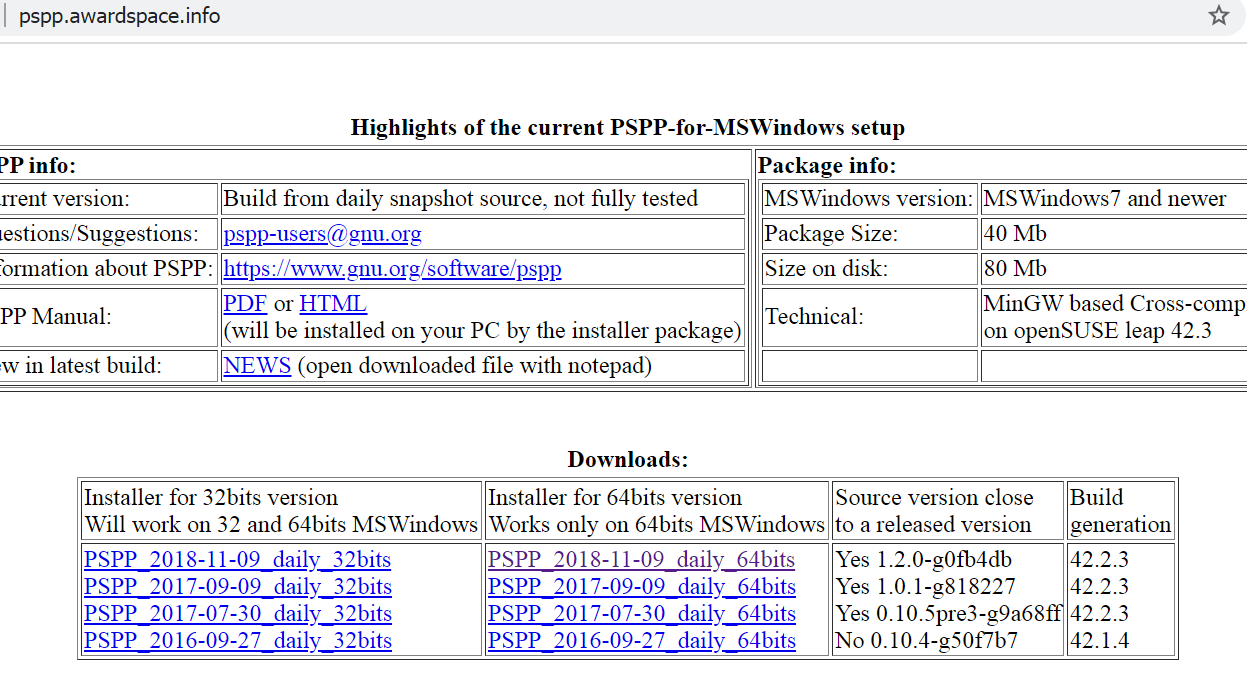
\includegraphics[width=0.65\linewidth]{images/psppdownload0}

Download the file

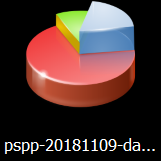
\includegraphics[width=0.25\linewidth]{images/psppdownload}

Install

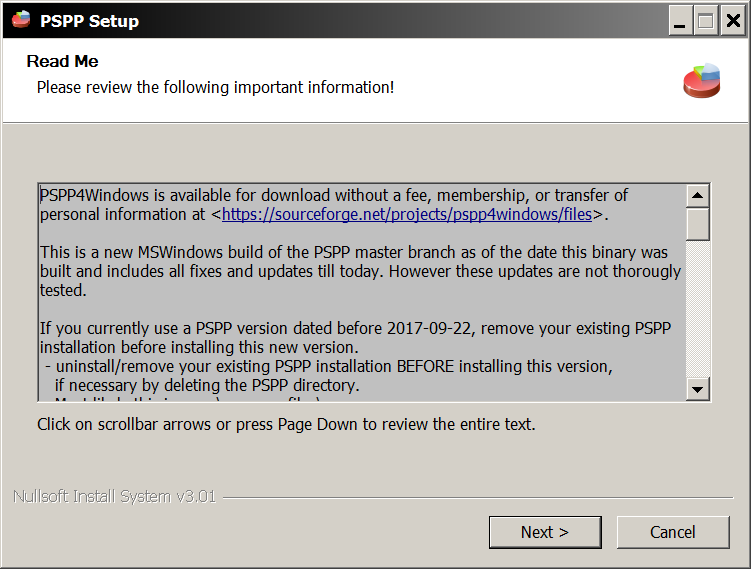
\includegraphics[width=0.65\linewidth]{images/psppinstall}

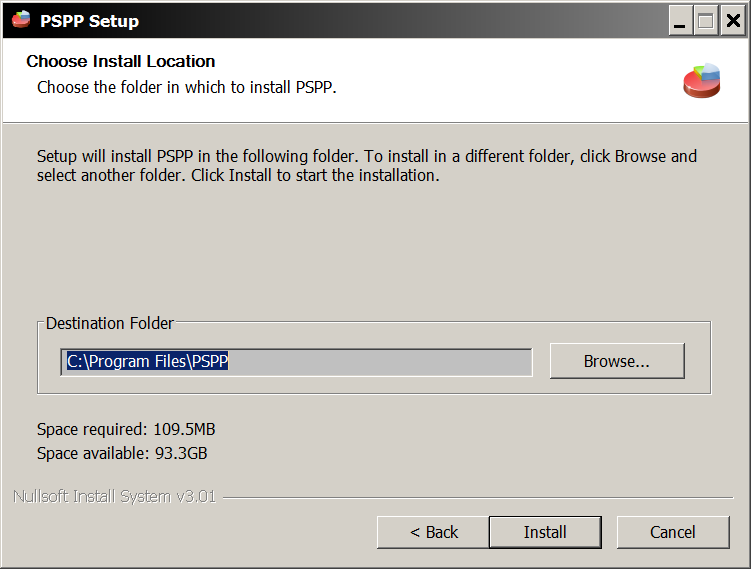
\includegraphics[width=0.65\linewidth]{images/psppinstall2}

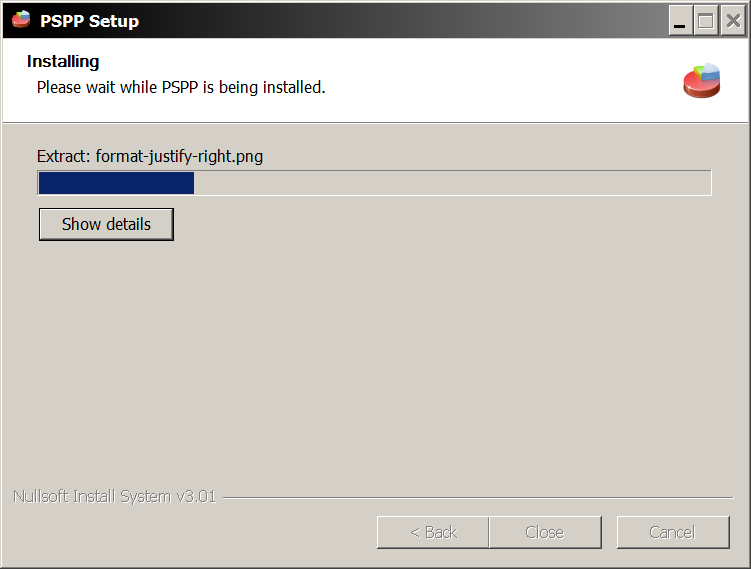
\includegraphics[width=0.65\linewidth]{images/psppinstall3}

Click the icon shorcut after installing

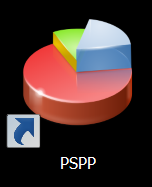
\includegraphics[width=0.25\linewidth]{images/psppicon}

\begin{itemize}
\tightlist
\item
  \textbf{Step 2}: Open PSPP
\end{itemize}

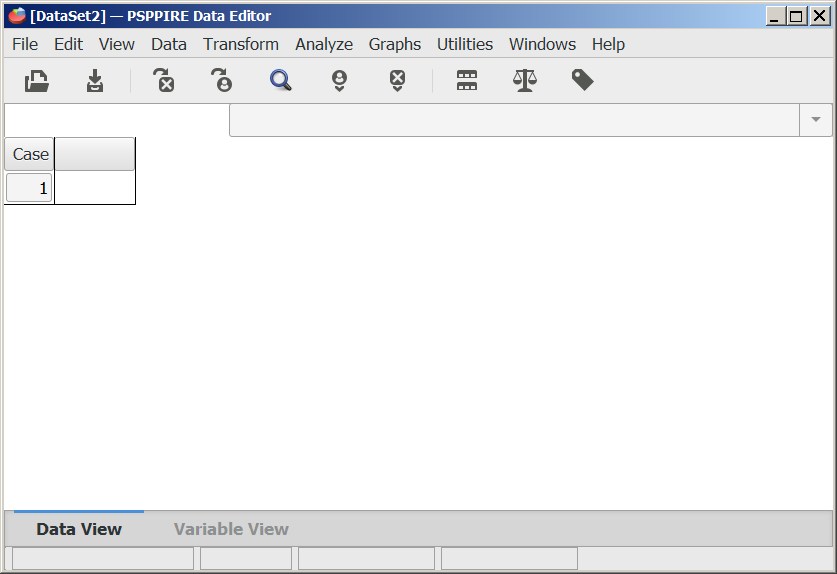
\includegraphics[width=0.65\linewidth]{images/abacus31}

\begin{itemize}
\tightlist
\item
  \textbf{Step 3}: Go to `file' menu and click `open'
\end{itemize}

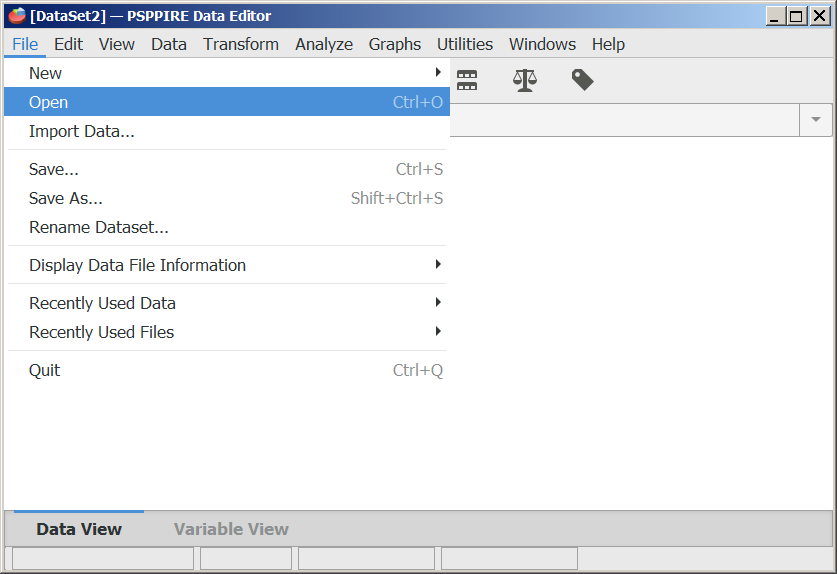
\includegraphics[width=0.65\linewidth]{images/abacus32}

\begin{itemize}
\tightlist
\item
  \textbf{Step 4}: Specify the \emph{readfile.sps} file from the `SAS\_SPSS' folder.
\end{itemize}

\includegraphics[width=0.65\linewidth]{images/abacus33}

You will see the following file:

\includegraphics[width=0.65\linewidth]{images/abacusX33}

\begin{itemize}
\tightlist
\item
  \textbf{Step 5}: Similar to before, change the directories as appropriate. Get rid of the extra lines of codes. Resulting codes are as follows (you can copy and replace the code in the file with the following codes):
\end{itemize}

\begin{Shaded}
\begin{Highlighting}[]
\NormalTok{file handle infile}\OperatorTok{/}\NormalTok{name =}\StringTok{ 'C:\textbackslash{}CCHS\textbackslash{}Data\textbackslash{}cchs_cycle3-1CD\textbackslash{}DATA\textbackslash{}hs.txt'}\NormalTok{.}
\NormalTok{data list file =}\StringTok{ }\NormalTok{infile notable}\OperatorTok{/}\NormalTok{.}
\NormalTok{include file =}\StringTok{ "C:\textbackslash{}CCHS\textbackslash{}Data\textbackslash{}cchs_cycle3-1CD\textbackslash{}SAS_SPSS\textbackslash{}Layouts\textbackslash{}hs\textbackslash{}hs_i.sps"}\NormalTok{.}
\NormalTok{include file =}\StringTok{ "C:\textbackslash{}CCHS\textbackslash{}Data\textbackslash{}cchs_cycle3-1CD\textbackslash{}SAS_SPSS\textbackslash{}Layouts\textbackslash{}hs\textbackslash{}hsvale.sps"}\NormalTok{.}
\NormalTok{include file =}\StringTok{ "C:\textbackslash{}CCHS\textbackslash{}Data\textbackslash{}cchs_cycle3-1CD\textbackslash{}SAS_SPSS\textbackslash{}Layouts\textbackslash{}hs\textbackslash{}hsvare.sps"}\NormalTok{.}
\NormalTok{include file =}\StringTok{ "C:\textbackslash{}CCHS\textbackslash{}Data\textbackslash{}cchs_cycle3-1CD\textbackslash{}SAS_SPSS\textbackslash{}Layouts\textbackslash{}hs\textbackslash{}hsmiss.sps"}\NormalTok{.}
\NormalTok{execute.}
\end{Highlighting}
\end{Shaded}

\includegraphics[width=0.65\linewidth]{images/abacusX34}

For Mac users, it should be as follows (e.g., \texttt{username} should be your user name, if you are saving under the path \texttt{"/Users/username/CCHS/Data/"}):

\begin{Shaded}
\begin{Highlighting}[]
\NormalTok{file handle infile}\OperatorTok{/}\NormalTok{name =}\StringTok{"/Users/username/CCHS/Data/cchs_cycle3-1CD/Data/hs.txt"}\NormalTok{.}
\NormalTok{data list file =}\StringTok{ }\NormalTok{infile notable}\OperatorTok{/}\NormalTok{.}
\NormalTok{include file =}\StringTok{ "/Users/username/CCHS/Data/cchs_cycle3-1CD/SAS_SPSS/Layouts/hs/hs_i.sps"}\NormalTok{.}
\NormalTok{include file =}\StringTok{ "/Users/username/CCHS/Data/cchs_cycle3-1CD/SAS_SPSS/Layouts/hs/hsvale.sps"}\NormalTok{.}
\NormalTok{include file =}\StringTok{ "/Users/username/CCHS/Data/cchs_cycle3-1CD/SAS_SPSS/Layouts/hs/hsvare.sps"}\NormalTok{.}
\NormalTok{include file =}\StringTok{ "/Users/username/CCHS/Data/cchs_cycle3-1CD/SAS_SPSS/Layouts/hs/hsmiss.sps"}\NormalTok{.}

\NormalTok{execute.}
\end{Highlighting}
\end{Shaded}

\begin{itemize}
\tightlist
\item
  \textbf{Step 6}: Run the codes.
\end{itemize}

\includegraphics[width=0.65\linewidth]{images/abacus35}

\begin{itemize}
\tightlist
\item
  \textbf{Step 7}: This is a large data, and will take some time to load the data into the PSPP data editor. \textbf{Be patient}.
\end{itemize}

\includegraphics[width=0.65\linewidth]{images/waitX}

Once loading is complete, it will show the `output' and `data view'.

\includegraphics[width=0.65\linewidth]{images/abacusNew}

\includegraphics[width=0.65\linewidth]{images/abacus36}

Note that, you will get error message, if your files were not in the correct path. In our example, the path was \texttt{"C:\textbackslash{}CCHS\textbackslash{}Data\textbackslash{}"} for the zip file content (see the previous steps).

\begin{itemize}
\tightlist
\item
  \textbf{Step 7}: You can also check the `variable view'.
\end{itemize}

\includegraphics[width=0.65\linewidth]{images/abacus37}

\begin{itemize}
\tightlist
\item
  \textbf{Step 8}: Save the data by clicking `File' and then `save as \ldots{}'
\end{itemize}

\includegraphics[width=0.65\linewidth]{images/abacus38}

\begin{itemize}
\tightlist
\item
  \textbf{Step 9}: Specify the name of the datafile and the location / folder to save the data file.
\end{itemize}

\includegraphics[width=0.65\linewidth]{images/abacus39}

\begin{itemize}
\tightlist
\item
  \textbf{Step 10}: See the SAV file saved in the directory.
\end{itemize}

\includegraphics[width=0.65\linewidth]{images/abacus40}

\begin{itemize}
\tightlist
\item
  \textbf{Step 11}: To save CSV format data, use the following syntax.
\end{itemize}

\begin{Shaded}
\begin{Highlighting}[]
\NormalTok{SAVE TRANSLATE}
  \OperatorTok{/}\NormalTok{OUTFILE=}\StringTok{"C:/CCHS/Data/cchs3b.csv"}  
  \OperatorTok{/}\NormalTok{TYPE=CSV}
  \OperatorTok{/}\NormalTok{FIELDNAMES      }
  \OperatorTok{/}\NormalTok{CELLS=VALUES.}
\end{Highlighting}
\end{Shaded}

Note that, for categorical data, you can either save values or labels. For our purpose, we prefer values, and hence saved with values here.

\includegraphics[width=0.65\linewidth]{images/abacus41}

\begin{itemize}
\tightlist
\item
  \textbf{Step 12}: See the CSV file saved in the directory extracted from PSPP.
\end{itemize}

\includegraphics[width=0.65\linewidth]{images/abacus42}

\hypertarget{option-3-processing-data-using-spss}{%
\subsection{Option 3: Processing data using SPSS}\label{option-3-processing-data-using-spss}}

Log into \href{https://ubc.onthehub.com}{ubc.onthehub.com} to download SPSS. With your CWL account, UBC students should be able to download it. UBC \href{https://it.ubc.ca/services/desktop-print-services/software-licensing/spss}{IT website for SPSS} says:

\texttt{The\ SPSS\ software\ license\ with\ UBC\ specifies\ that\ SPSS\ must\ only\ be\ used\ by\ UBC\ Faculty,\ Students,\ and\ Research\ Staff\ and\ only\ for\ Teaching\ and\ non-commercial\ Research\ purposes\ related\ to\ UBC.}

Both network (for UBC owened devices) or standalone / home versions (for non-UBC owened devices) should be available. Once downloaded, same process of importing CCHS data in PSPP can also be applied on SPSS (same syntax files should work). Let me know if that is not the case.

\hypertarget{processing-data-in-r}{%
\section{Processing data in R}\label{processing-data-in-r}}

\hypertarget{download-software}{%
\subsection{Download software}\label{download-software}}

\begin{itemize}
\tightlist
\item
  \textbf{Step 1}: Download either `R' from CRAN \href{https://www.r-project.org/}{www.r-project.org} or `R open' from Microsoft \href{https://mran.microsoft.com/open}{mran.microsoft.com/open}
\end{itemize}

\includegraphics[width=0.65\linewidth]{images/R03}

\includegraphics[width=0.65\linewidth]{images/R01}

\begin{itemize}
\tightlist
\item
  \textbf{Step 2}: Download RStudio from \href{https://www.rstudio.com/}{www.rstudio.com/}
\end{itemize}

\includegraphics[width=0.65\linewidth]{images/R02}

\begin{itemize}
\tightlist
\item
  \textbf{Step 3}: Open RStudio
\end{itemize}

\includegraphics[width=0.65\linewidth]{images/R04}

\hypertarget{import-export-and-load-data-into-r}{%
\subsection{Import, export and load data into R}\label{import-export-and-load-data-into-r}}

\begin{itemize}
\tightlist
\item
  \textbf{Step 1}: Set working directory
\end{itemize}

\begin{Shaded}
\begin{Highlighting}[]
\KeywordTok{setwd}\NormalTok{(}\StringTok{"C:/CCHS/Data/"}\NormalTok{) }\CommentTok{# or something appropriate}
\end{Highlighting}
\end{Shaded}

\begin{itemize}
\tightlist
\item
  \textbf{Step 2}: Read the dataset created from PSPP with cell values. We can also do a small check to see if the cell values are visible. For example, we choose a variable `CCCE\_05A', and tabulate it.
\end{itemize}

\begin{Shaded}
\begin{Highlighting}[]
\NormalTok{Hs <-}\StringTok{ }\KeywordTok{read.csv}\NormalTok{(}\StringTok{"cchs3b.csv"}\NormalTok{, }\DataTypeTok{header =} \OtherTok{TRUE}\NormalTok{)}
\KeywordTok{table}\NormalTok{(Hs}\OperatorTok{$}\NormalTok{CCCE_05A)}
\end{Highlighting}
\end{Shaded}

\includegraphics[width=0.65\linewidth]{images/abacus46}

\begin{itemize}
\tightlist
\item
  \textbf{Step 3}: Save the RData file from R into a folder \texttt{SurveyData}:
\end{itemize}

\begin{Shaded}
\begin{Highlighting}[]
\KeywordTok{save}\NormalTok{(Hs, }\DataTypeTok{file =} \StringTok{"SurveyData/cchs3.RData"}\NormalTok{)}
\end{Highlighting}
\end{Shaded}

\begin{itemize}
\tightlist
\item
  \textbf{Step 4}: See the RData file saved in the directory extracted from R.
\end{itemize}

\includegraphics[width=0.65\linewidth]{images/abacus43}

\begin{itemize}
\tightlist
\item
  \textbf{Step 5}: Close R / RStudio and restart it. Environment window within RStudio should be empty.
\end{itemize}

\includegraphics[width=0.65\linewidth]{images/abacus44}

\begin{itemize}
\tightlist
\item
  \textbf{Step 6}: Load the saved RData into R. Environment window within RStudio should have `Hs' dataset.
\end{itemize}

\begin{Shaded}
\begin{Highlighting}[]
\KeywordTok{load}\NormalTok{(}\StringTok{"SurveyData/cchs3.RData"}\NormalTok{)}
\end{Highlighting}
\end{Shaded}

\includegraphics[width=0.65\linewidth]{images/abacus45}

\hypertarget{demystifying-nhanes}{%
\chapter{Demystifying NHANES}\label{demystifying-nhanes}}

\hypertarget{overview}{%
\section{Overview}\label{overview}}

National Center for Health Statistics (NCHS) has been conducting surveys combining interviews with health/laboratory and physical examination studies since 1959. The end-product, recently known as, National Health and Nutrition Examination Surveys (NHANES) provide cross-sectional data of the health and nutrition of the United States population. This information source has been central to formulating nationwide public health policies and practices.

\hypertarget{survey-history}{%
\section{Survey history}\label{survey-history}}

Overall NHANES survey history

\includegraphics[width=0.65\linewidth]{images/g1}

\hypertarget{nhanes-datafile-and-documents}{%
\section{NHANES datafile and documents}\label{nhanes-datafile-and-documents}}

\hypertarget{file-format}{%
\subsection{File format}\label{file-format}}

The Continuous NHANES files are stored in the NHANES website as SAS transport file formats (.xpt). You can import this data in any statistical package that supports this file format.

\hypertarget{continuous-nhanes-components}{%
\subsection{Continuous NHANES Components}\label{continuous-nhanes-components}}

Continuous NHANES \href{https://www.cdc.gov/nchs/tutorials/NHANES/SurveyOrientation/DataStructureContents/Info1.htm}{components} separated to reduce the amount of time to download and documentation size:

\includegraphics[width=0.65\linewidth]{images/g2}

\hypertarget{public-release-excludes}{%
\subsection{Public release excludes}\label{public-release-excludes}}

The following data have not been released on the NHANES website as public release files due to confidentiality concerns:

\begin{itemize}
\tightlist
\item
  adolescent data on alcohol use,
\item
  smoking,
\item
  sexual behavior,
\item
  reproductive health and drug use
\end{itemize}

\hypertarget{combining-data}{%
\subsection{Combining data}\label{combining-data}}

\hypertarget{different-cycles}{%
\subsubsection{Different cycles}\label{different-cycles}}

It is possible to combine datasets from different years/cycles together in NHANES. However, NHANES is a cross-sectional data, and identification of the same person accross different cycles is not possible in the public resease datasets. For appending data from different cycles, please make sure that the variable names/labels are the same/identical in years under consideration (in some years, names and labels do change).

\hypertarget{within-the-same-cycle}{%
\subsubsection{Within the same cycle}\label{within-the-same-cycle}}

Within NHANES datasets in a given cycle, each sampled person has an unique identifier sequence number (variable \texttt{SEQN}) and therefore various data components:

\begin{itemize}
\tightlist
\item
  demographics,
\item
  dietary,
\item
  examination,
\item
  laboratory and
\item
  questionnaire
\end{itemize}

within same cycle can be merged.

\hypertarget{missing-data-and-outliers}{%
\subsection{Missing data and outliers}\label{missing-data-and-outliers}}

\citet{CDCfaq} recommends:

\begin{quote}
\begin{enumerate}
\def\labelenumi{\arabic{enumi}.}
\tightlist
\item
  ``As a general rule, if 10\% or less of your data for a variable are missing from your analytic dataset, it is usually acceptable to continue your analysis without further evaluation or adjustment. However, if more than 10\% of the data for a variable are missing, you may need to determine whether the missing values are distributed equally across socio-demographic characteristics, and decide whether further imputation of missing values or use of adjusted weights are necessary.''
\end{enumerate}
\end{quote}

\begin{quote}
\begin{enumerate}
\def\labelenumi{\arabic{enumi}.}
\setcounter{enumi}{1}
\tightlist
\item
  ``If you fail to identify `refusal' or `do not know' as types of missing data, and treat the assigned values for `refused' or `do not know' as real values, you will get distorted results in your statistical analyses. Therefore, it is important to recode `refused' or `don't know' responses as missing values (either as a period (.) for numeric variables or as a blank for character variables).''
\end{enumerate}
\end{quote}

\begin{quote}
\begin{enumerate}
\def\labelenumi{\arabic{enumi}.}
\setcounter{enumi}{2}
\tightlist
\item
  ``Outliers with extremely large weights could have an influential impact on your estimates. You will have to decide whether to keep these influential outliers in your analysis or not. It is up to the analysts to make that decision.''
\end{enumerate}
\end{quote}

\hypertarget{nhanes-documents}{%
\subsection{NHANES documents}\label{nhanes-documents}}

\includegraphics[width=0.65\linewidth]{images/g3}

\hypertarget{exercise-web}{%
\section{Exercise (web)}\label{exercise-web}}

\begin{itemize}
\tightlist
\item
  More information about \href{https://wwwn.cdc.gov/nchs/nhanes/tutorials/module2.aspx}{NHANES design}
\item
  Visit \href{https://wwwn.cdc.gov/Nchs/Nhanes/search/}{US CDC} and do a variable keyword search based on your research interest (e.g., arthritis).
\end{itemize}

\hypertarget{importing-nhanes-to-r}{%
\chapter{Importing NHANES to R}\label{importing-nhanes-to-r}}

This is a short instruction document of how to get NHANES dataset from the US CDC site to your RStudio environment. Once we bring the dataset into RStudio, the next step is to think about creating analytic dataset.

\hypertarget{nhanes-dataset}{%
\section{NHANES Dataset}\label{nhanes-dataset}}

National Center for Health Statistics (NCHS) conducts National Health and Nutrition Examination Survey (NHANES) (\citet{nhanes}). These surveys are designed to evaluate the health and nutritional status of U.S. adults and children. These surveys are being administered in two-year cycles or intervals starting from 1999-2000. Prior to 1999, a number of surveys were conducted (e.g., NHANES III), but in our discussion, we will mostly restrict our discussions to `continuous NHANES' (e.g., NHANES 1999-2000 to NHANES 2017-2018).

Witin the CDC website, continuous NHANES data are available in 5 categories:

\begin{verbatim}
- Demographics
- Dietary
- Examination
- Laboratory
- Questionnaire
\end{verbatim}

\hypertarget{accessing-nhanes-data}{%
\section{Accessing NHANES Data}\label{accessing-nhanes-data}}

In the following example, we will see how to download `Demographics' data, and check associated variable in that data.

\hypertarget{accessing-nhanes-data-directly-from-the-cdc-website}{%
\subsection{Accessing NHANES Data Directly from the CDC website}\label{accessing-nhanes-data-directly-from-the-cdc-website}}

NHANES 1999-2000 and onward survey datasets are publicly available at \href{https://wwwn.cdc.gov/nchs/nhanes/}{wwwn.cdc.gov/nchs/nhanes/}.

\includegraphics[width=0.65\linewidth]{images/n15}

\begin{itemize}
\tightlist
\item
  \textbf{Step 1}: Say, for example, we are interested about NHANES 2015-2016 surveys. Clicking the associated link in the above Figure gets us to the page for the cirresponding cycle (see below).
\end{itemize}

\includegraphics[width=0.65\linewidth]{images/n15demo}

\begin{itemize}
\tightlist
\item
  \textbf{Step 2}: There are various types of data available for this survey. Let's explore the demographic information from this clycle. These data are mostly available in the form of SAS `XPT' format (see below).
\end{itemize}

\includegraphics[width=0.65\linewidth]{images/xptsasdata}

\begin{itemize}
\tightlist
\item
  \textbf{Step 3}: We can download the XPT data in the local PC folder and read the data into R as as follows:
\end{itemize}

\begin{Shaded}
\begin{Highlighting}[]
\CommentTok{# install.packages("SASxport")}
\KeywordTok{require}\NormalTok{(SASxport)}
\KeywordTok{library}\NormalTok{(foreign)}
\NormalTok{DEMO <-}\StringTok{ }\KeywordTok{read.xport}\NormalTok{(}\StringTok{"SurveyData}\CharTok{\textbackslash{}\textbackslash{}}\StringTok{DEMO_I.XPT"}\NormalTok{)}
\end{Highlighting}
\end{Shaded}

\begin{verbatim}
## 
## Attaching package: 'foreign'
\end{verbatim}

\begin{verbatim}
## The following objects are masked from 'package:SASxport':
## 
##     lookup.xport, read.xport
\end{verbatim}

\begin{itemize}
\tightlist
\item
  \textbf{Step 4}: Once data is imported in RStudio, we will see the \texttt{DEMO} object listed under data window (see below):
\end{itemize}

\includegraphics[width=0.65\linewidth]{images/rdata}

\begin{itemize}
\tightlist
\item
  \textbf{Step 5}: We can also check the variable names in this \texttt{DEMO} dataset as follows:
\end{itemize}

\begin{Shaded}
\begin{Highlighting}[]
\KeywordTok{names}\NormalTok{(DEMO)}
\end{Highlighting}
\end{Shaded}

\begin{verbatim}
##  [1] "SEQN"     "SDDSRVYR" "RIDSTATR" "RIAGENDR" "RIDAGEYR" "RIDAGEMN"
##  [7] "RIDRETH1" "RIDRETH3" "RIDEXMON" "RIDEXAGM" "DMQMILIZ" "DMQADFC" 
## [13] "DMDBORN4" "DMDCITZN" "DMDYRSUS" "DMDEDUC3" "DMDEDUC2" "DMDMARTL"
## [19] "RIDEXPRG" "SIALANG"  "SIAPROXY" "SIAINTRP" "FIALANG"  "FIAPROXY"
## [25] "FIAINTRP" "MIALANG"  "MIAPROXY" "MIAINTRP" "AIALANGA" "DMDHHSIZ"
## [31] "DMDFMSIZ" "DMDHHSZA" "DMDHHSZB" "DMDHHSZE" "DMDHRGND" "DMDHRAGE"
## [37] "DMDHRBR4" "DMDHREDU" "DMDHRMAR" "DMDHSEDU" "WTINT2YR" "WTMEC2YR"
## [43] "SDMVPSU"  "SDMVSTRA" "INDHHIN2" "INDFMIN2" "INDFMPIR"
\end{verbatim}

\begin{itemize}
\tightlist
\item
  \textbf{Step 6}: We can open the data in RStudio in the dataview window (by clicking the \texttt{DEMO} data from the data window). The next Figure shows only a few columns and rows from this large dataset. Note that there are some values marked as ``NA'', which represents missing values.
\end{itemize}

\includegraphics[width=0.65\linewidth]{images/dataview}

\begin{itemize}
\tightlist
\item
  \textbf{Step 7}: There is a column name associated with each column, e.g., \texttt{DMDHSEDU} in the first column in the above Figure. To understand what the column names mean in this Figure, we need to take a look at the codebook. To access codebook, click the \texttt{\textquotesingle{}DEMO\textbar{}Doc\textquotesingle{}} link (in step 2). This will show the data documentation and associated codebook (see the next Figure).
\end{itemize}

\includegraphics[width=0.65\linewidth]{images/toc}

\begin{itemize}
\tightlist
\item
  \textbf{Step 8}: We can see a link for the column or variable \texttt{DMDHSEDU} in the table of content (in the above Figure). Clicking that link will provide us further information about what this variable means (see the next Figure).
\end{itemize}

\includegraphics[width=0.65\linewidth]{images/DMDHSEDU}

\begin{itemize}
\tightlist
\item
  \textbf{Step 9}: We can assess if the numbers reported under count and cumulative (from the above Figure) matches with what we get from the \texttt{DEMO} data we just imported (particularly, for the \texttt{DMDHSEDU} variable):
\end{itemize}

\begin{Shaded}
\begin{Highlighting}[]
\KeywordTok{table}\NormalTok{(DEMO}\OperatorTok{$}\NormalTok{DMDHSEDU)}
\end{Highlighting}
\end{Shaded}

\begin{verbatim}
## 
##    1    2    3    4    5    7    9 
##  619  511  980 1462 1629    2   23
\end{verbatim}

\begin{Shaded}
\begin{Highlighting}[]
\KeywordTok{cumsum}\NormalTok{(}\KeywordTok{table}\NormalTok{(DEMO}\OperatorTok{$}\NormalTok{DMDHSEDU))}
\end{Highlighting}
\end{Shaded}

\begin{verbatim}
##    1    2    3    4    5    7    9 
##  619 1130 2110 3572 5201 5203 5226
\end{verbatim}

\begin{Shaded}
\begin{Highlighting}[]
\KeywordTok{length}\NormalTok{(}\KeywordTok{is.na}\NormalTok{(DEMO}\OperatorTok{$}\NormalTok{DMDHSEDU))}
\end{Highlighting}
\end{Shaded}

\begin{verbatim}
## [1] 9971
\end{verbatim}

\hypertarget{accessing-nhanes-data-using-r-packages}{%
\subsection{Accessing NHANES Data Using R Packages}\label{accessing-nhanes-data-using-r-packages}}

\hypertarget{nhanesa}{%
\subsubsection{nhanesA}\label{nhanesa}}

\texttt{nhanesA} provides a convenient way to download and analyze NHANES survey data.

\begin{Shaded}
\begin{Highlighting}[]
\CommentTok{#install.packages("nhanesA")}
\KeywordTok{library}\NormalTok{(nhanesA)}
\end{Highlighting}
\end{Shaded}

\begin{itemize}
\tightlist
\item
  \textbf{Step 1}: Witin the CDC website, NHANES data are available in 5 categories

  \begin{itemize}
  \tightlist
  \item
    Demographics (\texttt{DEMO})
  \item
    Dietary (\texttt{DIET})
  \item
    Examination (\texttt{EXAM})
  \item
    Laboratory (\texttt{LAB})
  \item
    Questionnaire (\texttt{Q})
  \end{itemize}
\end{itemize}

To get a list of available variables within a datafile, we run the following command (e.g., we check variable names within \texttt{DEMO} data):

\begin{Shaded}
\begin{Highlighting}[]
\KeywordTok{library}\NormalTok{(nhanesA)}
\end{Highlighting}
\end{Shaded}

\begin{verbatim}
## Warning: package 'nhanesA' was built under R version 4.0.2
\end{verbatim}

\begin{Shaded}
\begin{Highlighting}[]
\KeywordTok{nhanesTables}\NormalTok{(}\DataTypeTok{data_group=}\StringTok{'DEMO'}\NormalTok{, }\DataTypeTok{year=}\DecValTok{2015}\NormalTok{)}
\end{Highlighting}
\end{Shaded}

\begin{verbatim}
##   FileName                              Description
## 1   DEMO_I Demographic Variables and Sample Weights
\end{verbatim}

\begin{itemize}
\tightlist
\item
  \textbf{Step 2}: We can obtain the summaries of the downloaded data as follows (see below):
\end{itemize}

\begin{Shaded}
\begin{Highlighting}[]
\NormalTok{demo <-}\StringTok{ }\KeywordTok{nhanes}\NormalTok{(}\StringTok{'DEMO_I'}\NormalTok{)}
\end{Highlighting}
\end{Shaded}

\begin{verbatim}
## Processing SAS dataset DEMO_I 	 ..
\end{verbatim}

\begin{Shaded}
\begin{Highlighting}[]
\KeywordTok{names}\NormalTok{(demo)}
\end{Highlighting}
\end{Shaded}

\begin{verbatim}
##  [1] "SEQN"     "SDDSRVYR" "RIDSTATR" "RIAGENDR" "RIDAGEYR" "RIDAGEMN"
##  [7] "RIDRETH1" "RIDRETH3" "RIDEXMON" "RIDEXAGM" "DMQMILIZ" "DMQADFC" 
## [13] "DMDBORN4" "DMDCITZN" "DMDYRSUS" "DMDEDUC3" "DMDEDUC2" "DMDMARTL"
## [19] "RIDEXPRG" "SIALANG"  "SIAPROXY" "SIAINTRP" "FIALANG"  "FIAPROXY"
## [25] "FIAINTRP" "MIALANG"  "MIAPROXY" "MIAINTRP" "AIALANGA" "DMDHHSIZ"
## [31] "DMDFMSIZ" "DMDHHSZA" "DMDHHSZB" "DMDHHSZE" "DMDHRGND" "DMDHRAGE"
## [37] "DMDHRBR4" "DMDHREDU" "DMDHRMAR" "DMDHSEDU" "WTINT2YR" "WTMEC2YR"
## [43] "SDMVPSU"  "SDMVSTRA" "INDHHIN2" "INDFMIN2" "INDFMPIR"
\end{verbatim}

\begin{Shaded}
\begin{Highlighting}[]
\KeywordTok{table}\NormalTok{(demo}\OperatorTok{$}\NormalTok{DMDHSEDU)}
\end{Highlighting}
\end{Shaded}

\begin{verbatim}
## 
##    1    2    3    4    5    7    9 
##  619  511  980 1462 1629    2   23
\end{verbatim}

\begin{Shaded}
\begin{Highlighting}[]
\KeywordTok{cumsum}\NormalTok{(}\KeywordTok{table}\NormalTok{(demo}\OperatorTok{$}\NormalTok{DMDHSEDU))}
\end{Highlighting}
\end{Shaded}

\begin{verbatim}
##    1    2    3    4    5    7    9 
##  619 1130 2110 3572 5201 5203 5226
\end{verbatim}

\begin{Shaded}
\begin{Highlighting}[]
\KeywordTok{length}\NormalTok{(}\KeywordTok{is.na}\NormalTok{(demo}\OperatorTok{$}\NormalTok{DMDHSEDU))}
\end{Highlighting}
\end{Shaded}

\begin{verbatim}
## [1] 9971
\end{verbatim}

\hypertarget{rnhanes}{%
\subsubsection{RNHANES}\label{rnhanes}}

\texttt{RNHANES} (\citet{RNHANES}) is another packages for downloading the NHANES data easily. Try yourself.

  \bibliography{book.bib}

\end{document}
